% \documentclass[pdflatex,11pt]{aghdpl}
% \documentclass{aghdpl}               % przy kompilacji programem latex
\documentclass[pdflatex,en]{aghdpl}  % praca w języku angielskim
% \usepackage[polish]{babel}
\usepackage[utf8]{inputenc}

% dodatkowe pakiety
\usepackage{enumerate}
\usepackage{listings}
\usepackage[lined,boxed,commentsnumbered]{algorithm2e}
\usepackage{graphicx}
\usepackage{caption}
\usepackage{subcaption}
\lstloadlanguages{TeX}

% for \url command
\usepackage{url}

\lstset{
  literate={ą}{{\k{a}}}1
           {ć}{{\'c}}1
           {ę}{{\k{e}}}1
           {ó}{{\'o}}1
           {ń}{{\'n}}1
           {ł}{{\l{}}}1
           {ś}{{\'s}}1
           {ź}{{\'z}}1
           {ż}{{\.z}}1
           {Ą}{{\k{A}}}1
           {Ć}{{\'C}}1
           {Ę}{{\k{E}}}1
           {Ó}{{\'O}}1
           {Ń}{{\'N}}1
           {Ł}{{\L{}}}1
           {Ś}{{\'S}}1
           {Ź}{{\'Z}}1
           {Ż}{{\.Z}}1
}

%---------------------------------------------------------------------------

\author{Krzysztof Styrc}
\shortauthor{K. Styrc}

\titlePL{Zarządzanie wiarygodnością i integralnością danych w sfederowanych zasobach cloud storage}
\titleEN{Managing data reliability and integrity in federated cloud storage}

\shorttitlePL{Zarządzanie wiarygodnością i integralnością danych w sfederowanych zasobach cloud storage} % skrócona wersja tytułu jeśli jest bardzo długi
\shorttitleEN{Managing data reliability and integrity in federated cloud storage}

\thesistypePL{Praca magisterska}
\thesistypeEN{Master of Science Thesis}

\supervisorPL{dr inż. Marian Bubak}
\supervisorEN{Marian Bubak Ph.D}

\consultancyPL{Piotr Nowakowski}
\consultancyEN{Piotr Nowakowski}

\date{2012}

\departmentPL{Katedra Informatyki}
\departmentEN{Department of Computer Science}

\facultyPL{Wydział Elektrotechniki, Automatyki, Informatyki i Elektroniki}
\facultyEN{Faculty of Electrical Engineering, Automatics, Computer Science and Electronics}

\acknowledgements{Tu będą podziękowania}



\setlength{\cftsecnumwidth}{10mm}

%---------------------------------------------------------------------------

\begin{document}

\titlepages

\tableofcontents
\clearpage

\chapter{Introduction}
\label{cha:introduction}

This chapter presents the overview and general objectives of this thesis.
The first section outlines the background and the concept of
assuring data reliability. Cloud storage availability and integrity challenges
are introduced in the following section. Next, we present the origin of
this work in the context of VPH-Share Cloud Platform. In the final section,
the high-level objectives of this thesis are described.
 
\section{Background and overview}
In the modern world of the 21st century the data and its vast volume
are ubiquitous. The total amount of global data stored to date is estimated
as 4 zettabytes ($4 \times 10^{21}bytes$) in 2013, almost $50\%$ more than in 2012 \cite{idc-data-growth}.
As long as computers spread to 
new domains and new computing paradigms -- as internet of things and big data
-- become a reality, the trend of exponential growth of data volume
will continue. The main sources of data are of various kind:

\begin{itemize}
\item \textbf{personal data} -- generated by and associated with people such as
images, videos, emails, documents etc, stored on privately held devices as
laptops, smartphones or digital cameras as well as by website owners in
big data centers,
\item \textbf{business data} -- generated by companies and corporations
that enables them to run and maintain their daily business,
\item \textbf{experimental data} -- generated by all kind of sensor and
experimental devices from weather stations, to particle accelerators, to
space satellites and stored on academic resources and scientific data centers.
\end{itemize}

It is an engineering challenge to fullfill storage requirements for current
data growth. Nowadays, we observe a rapid shift from privately owned and maintained
computer systems toward virtualized computer infrastructures provided as a service,
namely cloud computing. At least several commercial cloud infrastructure offerings 
provide access to virtualized computer systems at different level -- Infrastructure
as a Service (IaaS), Platform as a Service (PaaS) and Software as a Service (SaaS).
Low costs, high availability and scalability, decent performance degradation and 
seamless integration are often mentioned as major benefits by cloud adopters and
evangelists.\\

Digitalization brought new opportunities and advantages to the business and communities.
As a~result, many of them became strictly tied to their data as a major asset and
can no longer tolerate any data loss. Temporal data unavailability can also pose 
a~problem in domains such as medical care and flight services. With the promise
of scalable data storage, where everything can be stored or archived for future
needs, it is a burning issue to provide means of data loss prevention.\\

In general, the methods of data loss prevention can be divided into two groups:

\begin{enumerate}
\item \textbf{corruption or loss detection} -- that the data content is unavailable
or no longer correct,
\item \textbf{corruption or loss recovery} -- that after data corruption detection
we can recover its original properties of availability and integrity.
\end{enumerate}

A number of methods exist and are in widespread use nowadays. Storage hardware
solutions -- CDs, hard disks, etc -- utilize error correcting codes (ECC) to prevent
small scale errors on read/write operations. Network protocols and software packages
distribution use hash-based checksums to verify the integrity of the content. Data
backups and replication are universal way of enabling recovery from data loss.\\

Ideally, from the user point of view, data storage solution should provide highly
available and fault-tolerant access to the data and be free of data corruption and
unavailability problems. However, it often appears that the above-mentioned
criteria cannot be met in practice,
especially when relying on single service provider. Cloud service providers protect
their customers data with data replication to geographically distributed zones,
strong securitiy policies and infrastructure monitoring. Even though, recently
a~number of cloud failures occured, questioning the reliability of
cloud solutions. Malicious and accidental data corruption threats also require
attention.\\ 

The standard concept of checking data integrity is based on checksum verification.
It consists of two major steps -- initial setup and verification. The first step
concerns with initial data deployment and computing checksum metadata of the content
-- a hash.In the verification step the integrity checksums of the data are once more
computed and compared with the reference ones. In the scope of this thesis, we discuss
the means of providing data reliability, by which we mean both:

\begin{enumerate}
\item \textbf{availability} -- that the data is available to the requesting entity,
\item \textbf{integrity} -- that the data remains untouched by malicious or undesired
modifications.
\end{enumerate}

Managing data availability and integrity of data in cloud storage environment is the
subject of this thesis. As we mentioned above, to provide a solid way of assuring data
reliability we must address both data corruption detection and recovery. The idea is
to, apart from the internal cloud provider replication, replicate the data over multiple
cloud provider resources, continuously monitor its integrity and enable possibility to restore corrupted
entities from existing replicas. In case of irreparable corruption we should notify the
owner about the data problem. Replicating the data over cloud providers will build another
abstraction layer on top of cloud service and will allow to use them interchangeably in so
called federation of cloud storage. With federated approach we can easily detect cloud provider
failure and switch to another.

\section{Cloud storage data reliability challenges}

Over the last years, we observe a rapid shift from privately owned and maintained
storage resources toward cloud storage solutions. The cloud model of business become
popular and adopted by many organizations. The main driving forces of cloud computing
shift are low costs, high availability and scalability, decent performance degradation
and seamless integration. While the emerging trend determines a significant step forward 
in storage technology and brings a lot of advantages as data replication, no administration
costs, pay-as-you-use, SLA contracts -- it can appear challenging for ensuring data 
reliability. Remotely available resources introduce network transfer rates and latency issues,
while SLA contracts are mostly best-effort -- cloud provider will not charge fees if service
quality has not been met. Additionally, recent cloud storage failures or security break
reports shown that we cannot entrust our data to cloud providers entirely.\\
 
Classic checksum-based integrity verification methods are based on the whole content of data. It
poses a challenge to efficiently verify the integrity of vast volumes of data stored on remote resources,
where network transfer rates and latency comes into play. Additionally, cloud
storage providers charge fees not only for storage space used, but also for storage transfer.
Consequently, cloud storage data reliability methods should take these limitations into
consideration. It appears inevitable that cloud storage data integrity can be only provided with
some level of probability and has to be based on a fraction of the file. A part of this thesis main
objective is to select and implement a network-efficient method of ensuring data reliability.


\section{VPH-Share Cloud Platform context}
This thesis originates as a part of the VPH-Share project founded by European Commission
which brings together twenty international partners from academia, industry and healthcare,
led by University of Sheffield. Its main goal is to build a collaborative computing
environment and infrastructure where researchers from the domain of physiopathology of
the human body will work together on developing new medical simulation software. The inspiring
vision is to create a versatile environment for sharing of information -- tools, models and data
-- to work efficiently towards building a complete model of the human body.\\

The project has layered architecture divided into work packages distributed among consortium
members (see figure \ref{fig:dri-high-level}). The design is based on cloud computing middleware
-- a hybrid of commercial and private resources on top of hardware layer. Data and Compute
Cloud Platform is one of the main building blocks of the VPH-Share project. Its goal is to
develop and integrate a consistent service-based cloud infrastructure that will enable VPH
community to deploy basic components of VPH-Share application workflows (known as Atomic Services)
on the available computing resources and then enact workflows using these services. Access to the
services layer will be provided to system users through user interface(UI).

\begin{figure}[h!]
	\centering
	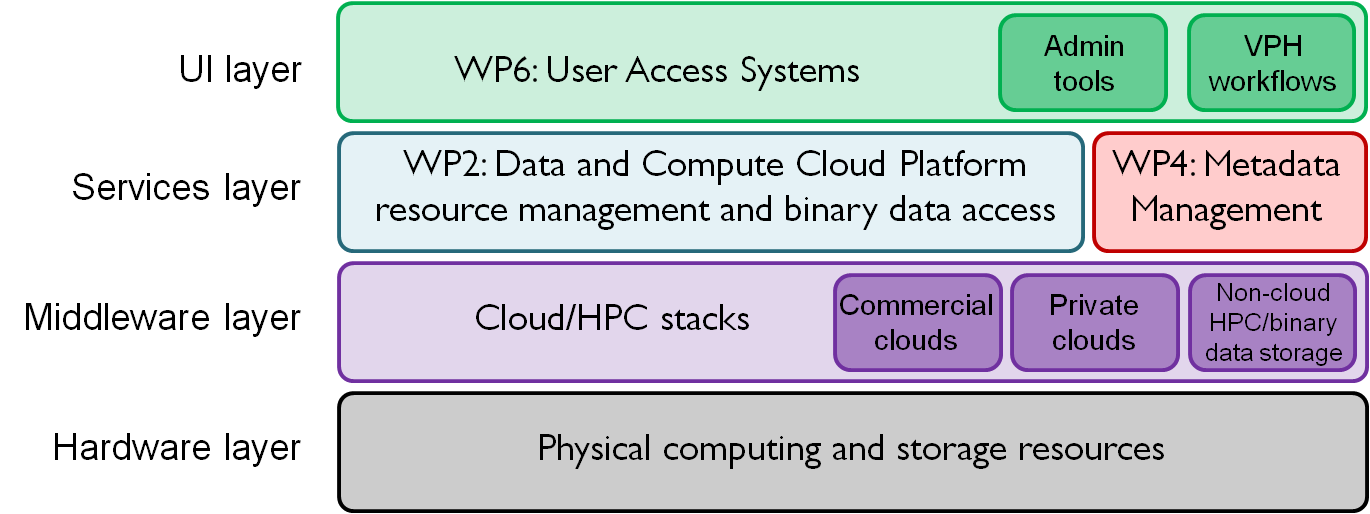
\includegraphics[width=0.8\textwidth]{images/vph-high-level.png}
	\caption{VPH-Share overview\\
	The project aims to build a collaborative computing environment
	for researchers of human body to work on developing new medical simulation software.
	Its design has layered architecture centered around service-based Data and Compute
	Cloud Platform built on top of hybrid cloud middleware, both commercial and private. The VPH-Share
	users use the platform through common user interface layer.}
	\label{fig:dri-high-level}
\end{figure} 


VPH-Share specifies three groups of users:
application providers, domain scientists and system administrators. Application providers
are responsible for developing and installing scientific applications and software packages.
Domain scientists are actual researchers of VPH community who will use and benefit from 
the platform. Finally, system administrators is a group of priviledged users who will
manage platform's hardware resources and will administer and maintain it.\\

According to the platform's design, data will be stored on federated cloud storage resources --
both commercial and private -- and available via common access layer. It is foreseen that stored
data volumes will be significant, but predominantly of static nature -- upon upload its content will
remain untouched. Additional measures should ensure data availability and integrity.As a result, two
of the key project's requirements regarding data storage and integrity are:

\begin{itemize}
\item \textbf{access to large binary data in the cloud} -- specified groups of users will
be able to query for and store binary data uploaded or generated by workflows within the platform, 
\item \textbf{data reliability and integrity} -- platform users will be able to tag datasets
for automatic availability and integrity monitoring, set validation and replication policies,
as well as receive notifications about data integrity violations.
\end{itemize}


\section{Objectives of this work}

As it was mentioned in the previous sections, there is a~need for creation of a~service that
will provide monitoring of data reliability and integrity (DRI) in federation of cloud storage
resources, in particular within VPH-Share Cloud Platform environment. The high-level objective of this
thesis is to design and implement such service that:

\begin{enumerate}
\item efficiently and  periodically monitor the integrity of the federated cloud storage,
\item notify the user about discovered data corruption in advance of data retrieval, 
\item provide possibility to restore corrupted data from replicas in other cloud providers.
\end{enumerate}

In this thesis, by efficient data integrity validation we mean network efficiency. Our goal is to minimize network
traffic required to validate a~file, while still be able to detect corruption on acceptable
level of probability.\\


\begin{figure}[h!]
	\centering
	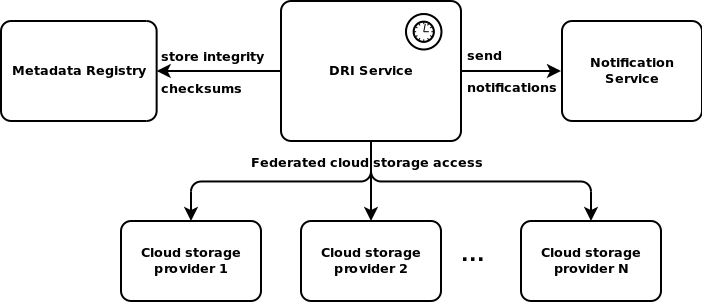
\includegraphics[width=0.8\textwidth]{images/DRI-objectives.png}
	\caption{DRI service is a~stateless web service within service-based VPH-Share Cloud Platform.
	Its main objective is periodical validation of data availability and integrity stored on
	federated cloud storage. All the integrity metadata is stored in metadata registry, while data access
	is perfomed via common federated cloud storage access layer to multiple cloud providers. Corruption
	or unavailability violations are sent to the user via Notification Service component.}
	\label{fig:dri-objectives}
\end{figure} 

At this point, the architecture of DRI service can be presented as a separate component within service-based 
environment that depends on other VPH-Share Cloud Platform core components visible in figure \ref{fig:dri-objectives}.
Conceptually, DRI service is a part of service-based VPH Cloud Platform architecture and provides
a~stateless web interface that enables managing data reliability (see figure \ref{fig:dri-objectives}).
To fullfill its responsibilities
DRI depends on a~number of other services. All of the service metadata regarding integrity checksums
and statuses, replication policies and federated cloud access is stored externally in metadata registry.
Data integrity and replication is performed on a~multiple cloud providers via common federated cloud
storage access layer. User notifcations are sent via external notification service.\\

DRI considers a~concept of dataset -- simply a set of files. Upon tagging dataset as managed DRI triggers
integrity checksums computation and stores them in metadata registry. As long as dataset remains managed
a~periodical availability and integrity verification takes place. When data corruption is detected the
user is notified about the errors via notification service and can restore the content from other replicas.



\chapter{Data integrity}
\label{cha:state_of_the_art}
High-quality data availability and integrity property is a must-have
requirement in many IT systems. A lot of enterprise and scientific effort
has been put into development of tools and methods that support this capability.
From cryptographic hash-based mechanisms that enable corruption discovery, to
replication and error-correcting codes for data recovery, to security
mechanisms preventing malicious data corruption. However, emerging trends in IT
solutions, as cloud computing, put new challenges in this area. The following
chapter presents the state of the art.\\

This chapter presents an introduction to a~set of topics connected with 
data integrity in cloud storage. In the first section we present
general methods and tools for ensuring data integrity which form
fundamanetal building blocks for more advanced methods. Further, we
describe cloud storage model, we focus on its origins and advantages, but
also discuss limitations of its interface and SLA contracts. In the last
section we dive into the subject of assuring data integrity in cloud
storage and present some emerging methods: proofs of retrievability (PORs)
and data integrity proofs (DIPs).



	\section{General methods and tools for ensuring data integrity}
	\label{classic-integrity-methods}
Providing a way to check the integrity of information transmitted over or
stored in an unreliable medium is a prime necessity in the world of open
computing and communications. The following section presents security building
blocks that enable data integrity assurance. The cryptographic hash functions
are core components of message authentication code algorithm to provide message
integrity and authenticate the message creator. Error correcting codes are 
commonly deployed to be able to retrieve the original data after partial
corruption.
 
		\subsection{Cryptographic hash functions}
A cryptographic hash function is a hash algorithm that maps a message of
arbitrary length to a fixed-length message digest (hash value). These
algorithms enable determination of a message's integrity: any change to the
message will, with high probability, result in a different message digest.
This property appears very useful as a building block in various security
constructions from generation and verification of digital signatures, to
message authentication codes, to generation of random numbers.\\ 

A cryptographic hash function is expected to have the following properties
\cite{nist-hash}:\\

\begin{itemize}
	\item \textbf{Collision resistance}: that it is computationally infeasible
	to find two different hash function inputs that have the same hash value.
	In other words, it is computationally infeasible to find $x$ and $x'$ for
	which $hash(x) = hash(x')$.
	\item \textbf{Preimage resistance}: that given a randomly chosen hash
	value, $hash\_value$, it is computationally infeasible to find an x so that
	$hash(x) = hash\_value$. This property is also called one-way property.
	\item \textbf{Second preimage resistance}: that it is computationally
	infeasible to find a second input that has the same hash value as any other
	specified input. That is, given an input $x$, it is computationally
	infeasible to find a second input $x'$ that is different from $x$, such
	that $hash(x) = hash(x')$.
\end{itemize}

Currently, the Secure Hash Standard (SHS) \cite{fips-shs} specifies five
approved hash algorithms: SHA-1, SHA-224, SHA-256, SHA-384 and SHA-512. Their
strengths of the security properties discussed above, vary significantly. While
one cryptographic hash function is suitable for one application, it might not
be suitable for other. The general trend is that the longer the message digest
(its hash), the stronger security guarantees, but also higher computational
complexity.\\

Additionally, the algorithms differ in terms of the size of the blocks and
words of data that are used during hashing or message digest sizes. They are
presented in table \ref{tab:hash-comparison}.

\begin{table}[h!]
\centering
\begin{tabular}{|l||c|c|c|c|}
	\hline
	Algorithm & Message Size (bits) & Block Size (bits) & Word Size (bits) & Message Digest Size (bits) \\ \hline \hline
	SHA-1   &  $< 2^{64}$ &  512 & 32 & 160 \\ \hline
	SHA-224 &  $< 2^{64}$ &  512 & 32 & 224 \\ \hline
	SHA-256 &  $< 2^{64}$ &  512 & 32 & 256 \\ \hline
	SHA-384 & $< 2^{128}$ & 1024 & 64 & 384 \\ \hline
	SHA-512 & $< 2^{128}$ & 1024 & 64 & 512 \\ \hline
\end{tabular}
\caption{Secure hash algorithm properties \cite{fips-shs}}
\label{tab:hash-comparison}
\end{table}

		\subsection{Error correcting codes}
An error-correcting code (ECC) is an algorithm for expressing a sequence of
numbers such that any errors which are introduced can be detected and corrected
(up to certain level) based on the remaining numbers. All error
correcting codes are based on the same basic principle: redundancy is added to
information in order to correct any errors that may occur in the process of
storage or transmission. In practice, the redundant symbols are appended to the
information symbols to obtain a coded sequence (codeword).\\

ECC can be divided into two classes:\\

\begin{itemize}
	\item \textbf{block codes}: that work on fixed-size blocks of predetermined
	size,
	\item \textbf{convolutional codes}: that work on bit streams of arbitrary
	length.
\end{itemize}

Among classical block codes the most popular are Reed-Solomon codes which are
in widespread use on the CDs, DVDs and hard disk drives. Hamming codes are
commonly used to prevent NAND flash memories errors. On the other hand,
convolutional codes are widely used in reliable data transfer such as digital
video, radio, mobile and satellite communication. Both block and convolutional
codes are often implemented in concatenation.\\

Apart from embedding ECC in the hardware solutions, they are also being applied
in software constructions to recover from eventual data corruption.

		\subsection{Message authentication codes}
A message authentication code (MAC) is an authentication tag (also called 
a~checksum) derived by applying an authentication scheme, together with 
a~secret key, to a message \cite{nist-hmac}. The purpose of a MAC is to
authenticate both the source of a message and its integrity without the use of
any additional mechanisms.\\

MACs based on cryptographic hash functions are known as HMACs. They have two
functionally distinct parameters: a message input and a secret key known only
to the message originator and intended receivers.\\

An HMAC function is used by the message sender to produce a value (the MAC)
that is formed by condensing the secret key and the message input. The MAC is
typically sent to the message receiver along with the message. The receiver
computes the MAC on the received message using the same key and HMAC function
as were used by the sender, and compares the result computed with the received
MAC. If the two values match, the message has been correctly received, and the
receiver is assured that the sender is a member of the community of users that
share the key \cite{nist-hmac}.\\

To compute a MAC over the data $text$ using the HMAC function with key $K$, the
following operation is performed \cite{nist-hmac}:

\begin{equation}
	MAC(text) = HMAC(K, text) = H(((K_{0} \oplus opad)||H((K_{0} \oplus ipad) || text)))
\end{equation}

where:

\begin{itemize}
	\item \textbf{$K_{0}$} -- the key $K$ after any necessary pre-processing to
	form a $B$ byte key,
	\item \textbf{$ipad$} -- inner pad, the byte $0x36$ repeated $B$ times,
	\item \textbf{$opad$} -- outer pad, the byte $0x5c$ repeated $B$ times,
	\item \textbf{$B$} -- block size (in bytes) of the input to the $H$ hash function,
	\item \textbf{$H$} -- an approved hash function.
\end{itemize}

The Internet Engineering Task Force (IETF) published a RFC document to describe
HMAC \cite{rfc2104}.\\

Apart from HMAC, a couple of other MACs have been proposed. Stinson
\cite{unconditional-mac} presented an unconditionally secure MAC based on 
encryption with a one-time pad. The cipher text of the message authenticates
itself as nobody else has access to the one-time pad. Lai et al.
\cite{stream-mac} proposed a MAC based on stream ciphers. In their algorithm,
a~provably secure stream cipher is used to split a message into two substreams
and each substream is fed into a linear feedback shift register (LFSR); the
checksum is the final state of the two LFSRs.\\

	\section{Cloud storage model}
	\label{cloud-model}
Cloud computing is an emerging IT trend toward loosely coupled networking of
computing resources. Its core feature is to move computing and data away from
desktop and portable PCs to large data centers and provide it as a service. The
popularity of this paradigm develops as it reduces IT expenses and provide
agile IT services to both, organisations and individuals. Additionally, users
are released from the burden of frequent hardware updates and costly
maintenance, while paying for cloud services on consumption basis.\\

While cloud computing represents the full spectrum of computing resources, this
work focuses on cloud storage services for archival and backup data. As it will
be shown, this technology, apart from its advantages, introduces many problems,
especially for ensuring data availability and integrity which may appear as
untrustworthy.   
		\subsection{General features}
Cloud storage is a model of broadband network access to virtualized pool of
storage resources on demand. In the spirit of cloud computing paradigm, it is 
mostly provided via REST/SOAP web service interface, however, other standard
protocols are used. Despite incompatibilities among various cloud storage
providers, as cloud computing gets more mature technology, their
interfaces begin to standardize. Storage Networking Industry Association (SNIA)
works toward developing a reference Cloud Data Management Interface (CMDI).\\

While different cloud storage solutions vary significantly, the following
common properties can be derived:

\begin{itemize}
	\item storage space is made up of many distributed resources, but still
	acts as one, virtualized layer,
	\item high fault-tolerance through redundancy and distribution of data,
	\item high data durability via object versioning,
	\item predominantly eventual consistency with regard to data replicas.
\end{itemize} 

Typically, public cloud providers expose storage space as object data store,
where data is organized into containers (or buckets). Each container consists
of data objects (files) on which standard create, read, update, delete (CRUD)
operations may be performed. Additional metadata is appended to containers and
data objects such as name, size, creation/modification date or hash checksum.\\

Amazon Simple Storage Service (S3) \cite{amazon-s3}, 
Rackspace Cloud Files \cite{rackspace-cloud} and
Google Cloud Storage \cite{google-cloud} are the most popular representatives
of the illustrated cloud storage model. Despite the increasing popularity of
public cloud storage providers, hybrid and private cloud solutions do exist,
Openstack Swift \cite{openstack-cloud} and 
Eucalyptus Cloud \cite{eucalyptus-cloud} to name just a few.\\

		\subsection{Interface and API}
Current cloud storage systems mostly provide REST/SOAP web service interface to
access the resources, in the spirit of Service Oriented Architecture (SOA)
paradigm. While this thesis focuses on this method of access and its
consequences, other providers expose different types of interface. Some of
them are presented in figure \ref{fig:cloud-access} with concrete examples of
solutions \cite{cloud-storage-anatomy}.

\begin{figure}[h!]
	\centering
	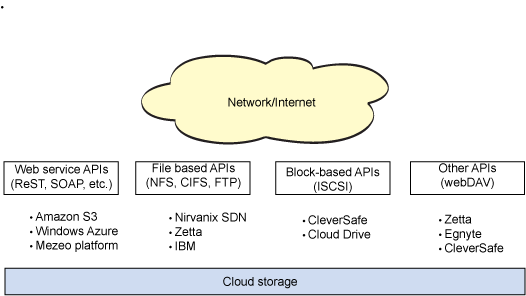
\includegraphics[width=0.8\textwidth]{images/cloud-access.png}
	\caption{Cloud storage access methods \cite{cloud-storage-anatomy}}
	\label{fig:cloud-access}
\end{figure}

Despite the fact that web service interfaces enable loose coupling and
technology interoperability, they require integration code with an application.
Many multi-cloud libraries were created to enable interoperability across
similar cloud services on a higher level of abstraction 
\cite{cloud-federation}. Their goal is to establish basic and uniform cloud
storage access layer at the API level \cite{jclouds, libcloud}.\\

Typically, cloud storage interfaces provide API to query, access and manage
stored data, which can be divided into the following groups
\cite{amazon-s3, rackspace-cloud, google-cloud, openstack-cloud, 
eucalyptus-cloud}:\\

\begin{itemize}
	\item \textbf{Operations for authentication}: to secure the access to
	cloud storage data (mostly via token-based authentication),  
	\item \textbf{Operations on the account}: to operate on account metadata
	such as managing existing containers and additional provider-specific data
	services,
	\item \textbf{Operations on the container}: to manage container policy, 
	versioning, ACLs, lifecycle and location,
	\item \textbf{Operations on the data objects}: to enable CRUD operations.
\end{itemize} 

There exists a growing trend to adjust provider-specific interfaces with the
SNIA reference model \cite{amazon-s3, rackspace-cloud, openstack-cloud}.
		
		\subsection{Service Level Agreement}
To provide high quality of service, cloud storage providers widely guarantee
Service Level Agreement (SLA) contracts. These are mostly related to service
availability during the billing cycle. The service downtime is considered as
cloud network error or response errors to a valid user requests. Currently,
most of the providers guarantee the availability level of $99.9\%$ of the time
\cite{amazon-s3, rackspace-cloud, google-cloud}.\\

However, if the provider will fail to provide a guaranteed level of service,
the appriopriate percentage of the credit is returned to the client. In this
sense, cloud storage should be still treated as best-effort. IT systems that
demand uninterrupted operation simply cannot entirely rely on it.\\

Moreover, eventual consistency model is inherently embedded into the
overwhelming majority of cloud storage architectures, which places new problems
to the solutions, where strict data consistency is a crucial requirement
\cite{metastorage, cloud-federation}. Besides eventual consistency, SLA
contracts still only address the service availability, while omitting data
integrity or retrievability speed issues. Even though, cloud storage service
with described limitations still fit to the vast number of market 
applications.\\

Customers who require a higher data availability and integrity guarantees,
still need to seek for hybrid solutions and develop sophisticated layers on
top of existing infrastructure to meet their demands.

		\subsection{Constraints and limitations}
Cloud storage architecture presented in previous section exhibit many
advantages to potential users. Nevertheless, it also introduces a couple of
drawbacks for demanding solutions.\\

The most striking consequence of cloud storage, is that data is stored remotely
on provider's resources and user has very limited possibilities to monitor or
check its data through abstract access layer. Even small security vulnerability
may compromise the data of all users in public cloud model.\\

As it was shown in previous subsection, cloud SLA contracts still lack strong
availability and integrity guarantees, rather than cost-return policy. Even
though cloud storage is perceived as superb technology, a couple of serious
downtimes have been reported in the last years. Amazon S3 users experienced
several unavailability and data corruption periods \cite{amazon-downtimes},
while Google Gmail lost data of thousands of accounts \cite{gmail-downtime} and
Google Docs enabled unauthorized access to the stored documents 
\cite{docs-downtime}.\\

Cloud storage REST/SOAP interfaces are flexible and rich in capabilities, but
when accessed remotely outside of cloud compute resources, they suffer from
network latency for each HTTP request. Downloading a fragment of a file pose
another challenge. It is mostly achieved by setting HTTP Range parameter to the
desired value. However, only single range value is permitted. It is particularly
problematic for data integrity monitoring protocols (presented in the next
section) as they request a lot of small file's blocks, and for each block 
a~separate HTTP request has to be sent, which means increased network
overhead.\\

Moreover, cloud storage solutions lack user's code execution capability over
stored data. The data has to be downloaded in order to perform computation. It
makes present data integrity monitoring protocols impractical and inefficient,
because they assume computation capability on the prover's side.

\section{Approaches to data integrity in cloud storage}
\label{cloud-integrity-approaches}
One of the fundamental goals of cryptography is data integrity protection.
Primitives such as digital signatures and message-authentication codes (MACs),
described in section \ref{classic-integrity-methods}, were created to allow
an entity in possession of a file $F$ to verify that it has not been tampered
with. The simplest way is to use keyed hash function $h_{k}(F)$ to compute and
store a hash value along with secret, random key $k$ prior to archiving a file.
To verify that the prover (remote server, cloud provider) possess $F$, the
verifier releases key $k$ and asks the prover to compute and return $h_{k}(F)$.
By using multiple keys with their corresponding hash values, the verifier can
perform multiple, independent checks. However, this approach introduces high
resource overhead. It requires the verifier to store large number
of hash values and the prover to read the entire file for every proof.\\

A more challenging problem is to enable verification of the integrity of $F$
without knowledge of the entire file's contents. It was firstly described in
general view by Blum et al. \cite{memory-correctness}, who presented efficient
methods for checking the correctness of program's memory. Following works
concerned dynamic memory-checking in a range of settings. For instance, Clarke
et al. \cite{clarke} consider the case of checking the integrity of operations
performed on an arbitrarily-large amount of untrusted data, when using only 
a~small fixed-sized trusted state. Their construction employ an adaptive
Merkle hash-tree over the contents of this memory. However, Naor and Rothblum
showed that online memory checking may be prohibitively expensive for many
applications \cite{omc-complexity}. This implies that applications requiring
memory checking should make cryptographic assumptions, or use an offline
version of the problem.\\

Unauthorized modifications to portions of files can be detected by
cryptographic integrity assurance upon their retrieval. But in its basic form
it does not enable such detection capability prior to the retrieval, what many
other schemes aim to provide.\\

One of the mostly developed model of ensuring integrity of remotely stored data
is the proofs of retrievability (POR). The first formal description of POR
protocol was proposed by Juels and Kaliski \cite{por}. In their scheme,
the client applies error-correcting code and spot-checking to ensure both
possession and retrievability of files. Shaham et al. \cite{compact-por}
achieve POR scheme with full proofs of security and lower communication
overhead. Bowers et al. \cite{por2} simplify and improve the framework and
achieve lower storage overhead as well as higher error tolerance. Later on, 
they extend it to distributed systems \cite{hail}. However, all these schemes
are focusing on static data. Before outsourcing the data file $F$ 
a~preprocessing steps are applied. Every change to the contents of $F$ require
re-processing, which introduces significant computation and communication
complexity. Stefanov et al. \cite{iris} propose an authenticated file-system
for outsourcing enterprise data to the untrusted cloud service providers with
the first efficient dynamic POR.\\

Atenise et al. \cite{pdp} presented the provable data possession (PDP) model
in order to verify if an untrusted server stores a client's data without file
retrieval. Key components of their scheme are public key based homomorphic
verifiable tags. In the subsequent work, Atenise et al. \cite{pdp2} described
a PDP scheme that uses only symmetric key cryptography. As a result, they
achieved lower performance overhead.\\

A couple of practical implementations for remote integrity assurance have been
developed. Bowers et al. \cite{hail} designed HAIL (High Availability and
Integrity Layer) which takes advantage of data distribution over a set of
servers to achieve efficient POR-like scheme. Shraer et al. \cite{venus}
created Venus, a scheme that guarantees integrity and consistency for a group
of clients accessing a remote storage provider. Venus ensures that each data
object read by any client has previously been written by some client.
Additionally, it protects against retrieving older version of the object.
Bessani et al. \cite{depsky} implemented DEPSKY, a system that improves the
availability, integrity and confidentiality of information stored in the cloud
through encryption, encoding, and replication of data on diverse clouds that
form cloud-of-clouds.\\

In the following subsections we examine exhaustively a couple of schemes
mentioned above. We present their architecture, advantages and limitations.

\subsection{Proofs of retrievability}
In a POR \cite{por, por2} protocol, a file is encoded by a client before
deploying it on cloud storage for archiving. Then, it employs
bandwidth-efficient challenge-response scheme to probabilistically guarantee
that a file is available at remote storage provider. Most of POR protocols 
proposed to date, use the technique of spot-checking in the challenge-response
protocol to detect data corruption. In each challenge, a subset of file blocks
is verified, and the results of a computation over these blocks is returned to
the client. The returned results are checked using the original checksums
embedded into the file at encoding time.\\

The primary POR-like protocol we consider in detail, was proposed by Juels and
Kaliski \cite{por} -- a MAC-based POR scheme. In this approach, they firstly
preprocess the file $F$ by applying error-correcting codes and MAC checksums
in the following steps:

\begin{enumerate}
	\item \textbf{Error correction}: the file is divided into $b$ blocks of the
	same length and apply an $(n,k,d)$-error correcting code,
	which expands each chunk of size $k$ into size $n$ and is able to recover
	from up to $d-1$ errors. The resulting file is denoted as $F'$.
	\item \textbf{Encryption}: the file with appended ECCs is encrypted.
	\item \textbf{MAC computation}: a $m$ number of blocks are selected in
	$F''$, their MACs computed and appended to the file.
	\item \textbf{Permutation}: of file blocks to secure appended MACs against
	corruption.
\end{enumerate}

The graphical presentation of the process is depicted in figure \ref{fig:por-modified-file}.\\

\begin{figure}[h!]
	\centering
	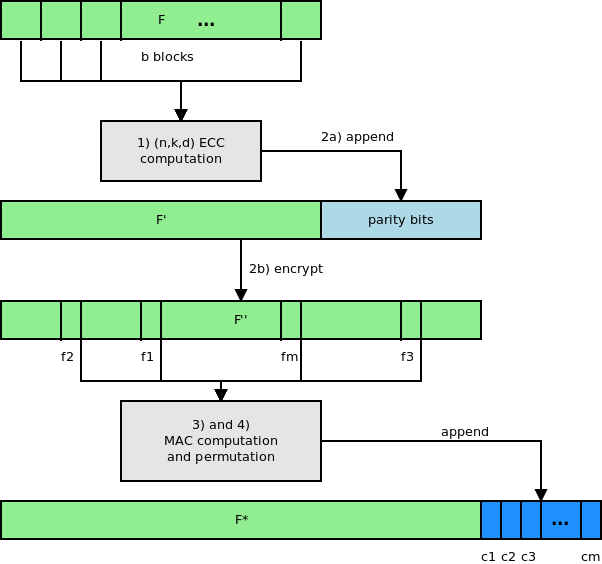
\includegraphics[width=0.8\textwidth]{images/por-schematic.png}
	\caption{Schematic presents POR based file encoding. Firstly (1), the file is divided into
	$b$ blocks and error correcting codes are applied to each of the block. Then (2), the
	parity bits are appended and the resulting file is encrypted. Finally (3,4), $m$ blocks of the encrypted
	file are selected, their MACs computed and appended to the file in permuted sequence. The resulting
	file is stored in archive \cite{por}.}
	\label{fig:por-modified-file}
\end{figure}

In the same paper \cite{por}, Juels and Kaliski proposed a sentinel-based POR
scheme. Similarily to the MAC-based approach it utilizes ECCs, but rather than
chosing MAC blocks it embeds sentinels in random positions in $F$, sentinels
being randomly constructed values. It is important that sentinels shall be 
indistinguishable from the encrypted file contents. The scheme consists of the
following steps:

\begin{enumerate}
	\item \textbf{Error correction}: the file is divided into $b$ blocks of the
	same length and apply an $(n,k,d)$-error correcting code,
	which expands each chunk of size $k$ into size $n$ and is able to recover
	from up to $d-1$ errors. The resulting file is denoted as $F'$.
	\item \textbf{Encryption}: the file with appended ECCs is encrypted.
	\item \textbf{Sentinel creation}: the randomly constructed sentinels are
	embedded in random positions in $F'$
	\item \textbf{Permutation}: which randomizes sentinel positions.
\end{enumerate}

In both approaches, if the prover has modified or deleted a substantial 
$e$-portion of $F$, then with high probability, also change roughly an
$e$-fraction of MAC-blocks or sentinels, respectively. It is therefore unlikely
to respond correctly to the verifier. Upon file retrieval, the user verifies
file's checksum. If it is not valid, then it starts file recovery based on
stored ECCs.\\

Of course, application of an error-correcting (or erasure) code and insertion
of sentinels enlarges $F^{*}$ beyond the original size of the file F. The
expansion induced by both POR protocols, however, can be restricted to a modest
percentage of the size of F. Importantly, the communication and computational
costs of the protocols are low.\\

The obvious advantage of the presented schemes is that they can be
parameterized.\\

Subsequent POR works \cite{compact-por, por2, hail, venus, iris} introduced
further optimizations to the solution described. The most important are:
moving MAC computation to the prover side and precomputing partial checksum
values.\\

However, POR-like schemes are not free from drawbacks. The primary limitation
is that preprocessing phase introduces non-negligible computational overhead.
Moreover, it requires storage of file $F$ in modified form. What is even more
problematic, it assumes that storage service provides user's code execution
capability, which is not true for current cloud storages 
(see section \ref{cloud-model}). For this reason, practical POR-like
implementation would require moving prover logic for computing 
challenge-response queries to the verifier. As a consequence, each access to
the portion of a file (MAC block or sentinel) would require separate HTTP
request. As many such accesses are performed per each file, it would be
impractical (except for large files, for which hundreds of short HTTP requests
would be faster than downloading the entire file).

\subsection{Data integrity proofs}
Data integrity proof (DIP) \cite{dip} is a protocol, which just like POR, aims
to assure that the remote archive poses the data. Unlike POR schemes, it does
not involve any modifications to the stored file. The client before storing
data file $F$, preprocesses it to create suitable metadata, which is used in
the later stage of data integrity verification. The preprocessing stage
consists of the following steps:

\begin{itemize}
	\item \textbf{Generation of metadata}: the file $F$ in divided into $n$
	blocks that each are $m$ bits length. Then, for each data block, a set of
	$k$ out of $m$ bits are selected. The value of $k$ is in the choice of the
	verifier and is a secret known only to him. Therefore, we get $n*k$ bits in
	total.
	\item \textbf{Encrypting the metadata}: each of the metadata from the data
	blocks, is encrypted by using a suitable algorithm and concatenated.
	\item \textbf{Appending the metadata}: all the metadata are appended to the
	file $F$, however, they can be also stored in the verifier.
\end{itemize}

The graphical presentation of the process is depicted in figure \ref{fig:dip-schematic}.\\

\begin{figure}[h!]
	\centering
	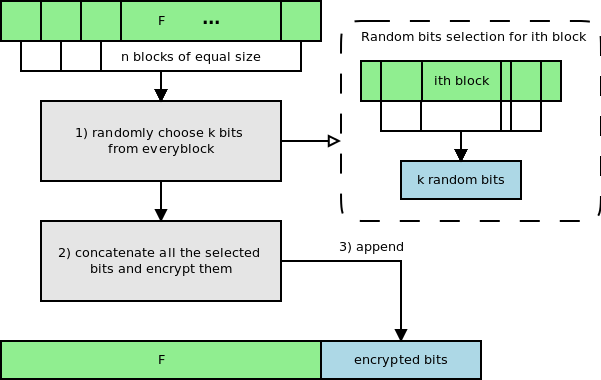
\includegraphics[width=0.8\textwidth]{images/dip-schematic.png}
	\caption{Schematic presents DIP based file encoding. Firstly (1), the file is
	divided into $n$ blocks of equal size and $k$ randomly chosen bits are selected
	out of each block. Then (2), concatenated bits from all of the blocks are encrypted
	and appended to the file $F$ \cite{dip}.}
	\label{fig:dip-schematic}
\end{figure}

To verify $F$ integrity, the verifier utilizes challenge-response mechanism. In
each challenge, it verifies a~single block $i$ specifing the positions of the
$k$ selected bits and retrieves encrypted metadata for this block to compare
the values. Any mismatch between the two would mean a loss of the integrity of
the clients data at the cloud storage.\\

While DIP scheme seems trivial, it eliminates a couple of disadvantages of the
POR approach. Firstly, data integrity assurance does not require any
modifications to the stored file, but also prevents the data recovery
capability by ECC. It also exhibits negligible computational overhead.
However, it still either assumes user's code execution capability by cloud
provider or requires large number of accesses to non-continuous data fragments.
Such data acceses are performed in separate HTTP requests in the current
cloud storages (see section \ref{cloud-model}), which is practically
infeasible.\\ 

\section{Summary}
In this chapter an important topics regarding data integrity and cloud storage were presented.
General methods and tools for ensuring data integrity such as cryptographic hash functions,
error correcting codes and message authentication codes were discussed. They form a set of
fundamental building blocks and patterns used in more advanced methods. Its understanding 
is crucial in further discussion on data integrity throughout this thesis. Further, the
overview of cloud storage model was presented. We focused on describing its origins in connection
with advantages which it brings in numerous applications. The discussion also includes the
high-level description of cloud storage interface and SLA contracts. We also stress the contraints
and limitations of moving the data to the cloud. Shortly, recent cloud providers failure reports
and the best-effort SLA contracts question the applicability of cloud storage in areas
such as medical care and flight services. In the last section, we extensively discuss current
approaches to data integrity in the cloud. We mainly focused on two developing schemes: proofs
of retrievability (PORs) and data integrity proofs (DIPs), but also mention other solutions and
improvements. 

\chapter{Data reliability and integrity service}
\label{cha:architecture}
This chapter presents the architecture of Data Reliability and Integrity (DRI)
service. It starts by describing the environment of VPH-Share Cloud Platform 
which specifies requirements under which DRI operates. Then it defines its 
design and interfaces with other parts of the system. At the end, the core 
validation heuristic algorithm is presented.

\section{Data and Compute Cloud Platform context}
\label{cloud-platform}
VPH-Share Data and Compute Cloud Platform project aims to design, implement,
deploy and maintain cloud storage and compute platform for application deployment
and execution. The tools and end-user services within the project will enable
researchers and medical practitioners to create and use their domain-specific
workflows on top of the Cloud and high-performance computing infrastructure.
In order to fulfill this goal, Cloud Platform will be delivered as consistent
service-based system that enables end users to deploy the basic components of
the VPH-Share application workflows (known as Atomic Services) on the available
computing resources and then enact workflows using these services.

\subsection{VPH-Share groups of users}
\label{vph-users}
VPH-Share project identifies three specific groups of users \cite{vph-deliverable-2-2}:

\begin{enumerate}
\item \textbf{Application providers} -- people responsible for developing and
installing scientific applications and software packages, typically IT experts
who collaborate with domain scientists and translate their requirements into
executable software.
\item \textbf{Domain scientists} -- actual researchers of the VPH community who
stand to benefit from access to scientific software packages provided by the 
platform. They will require the ability to access the applications in a~secure
and convenient manner via graphical interfaces provided on top of Cloud Platform.
\item \textbf{System administrators} -- priviledged users with ability to manipulate
and assign the available hardware resources to the project and define security/access
policies for other user groups. They will also make sure that the platform remains
operational by taking advantage of notification mechanisms built into the system.
\end{enumerate}

\subsection{Cloud platform architecture overview}

The general overview of Cloud Platform architecture with interactions to other parts of
the VPH-Share is illustrated in figure \ref{fig:vph-architecture}. Master UI (web portal) enables
coarse-grained invocations of the underlying core services to the specified groups of
end-users described in section \ref{vph-users}. The Cloud Platform itself will be deployed on
available cloud and physical resources.

\begin{figure}[h!]
	\centering
	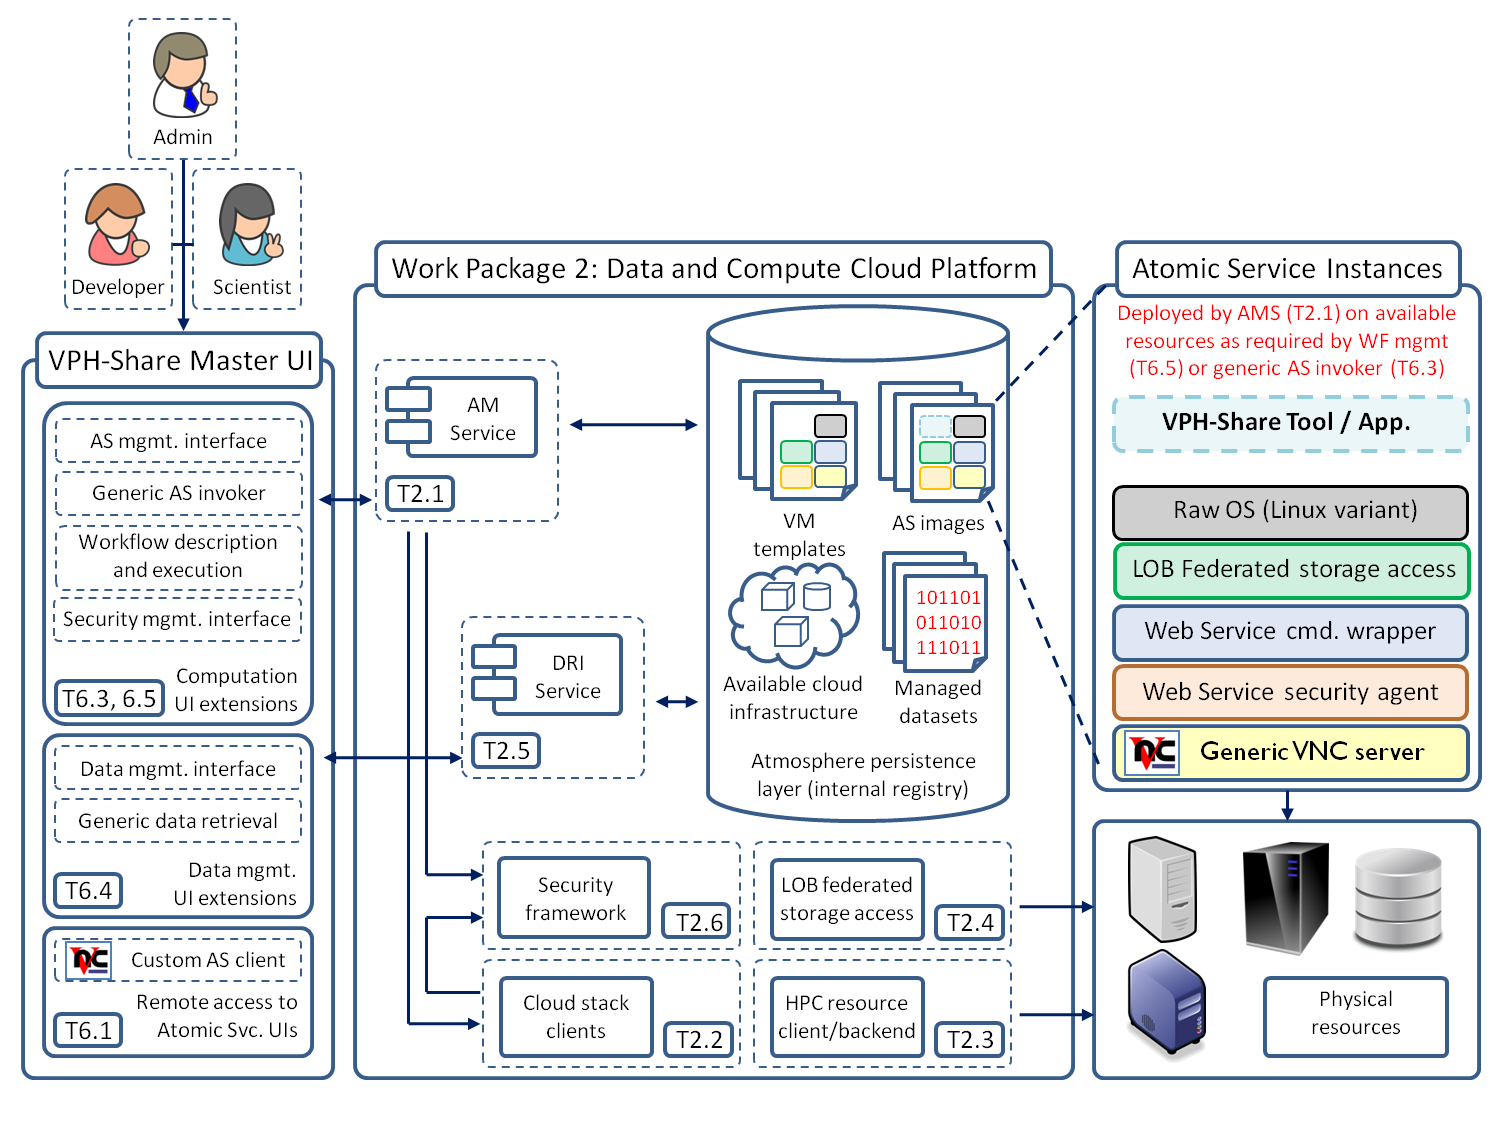
\includegraphics[width=\textwidth]{images/vph-architecture.png}
	\caption{VPH-Share Platform architecture. Specified groups of users are provided with
	functionalities of Cloud Platform through Master user interface (UI) which enables
	coarse-grained invocations of the underlying core services. Data and Compute Cloud
	Platform consists of loosly-coupled services responsible for exposing different platform
	functionalities such as federated storage access (T2.4), data integrity monitoring
	(2.5) etc. Services are deployed as Atomic Service instances (simply a~VM with add-ons).
	The platform is built on top of cloud computing resources \cite{vph-deliverable-2-2}.}
	\label{fig:vph-architecture}
\end{figure}

Cloud Platform interally consists of many loosly-coupled components deployed as Atomic Service
Instances (see section \ref{atomic-service}). Data storage is an essential functionality of
the Platform. It is achieved by
federated cloud storage which makes use of both, cloud and other storage
resources with redundancy and is accessible through common data layer --
LOBCDER service. Atmosphere Internal Registry (AIR) serves as
centralised metadata storage component which enables integration between 
loose-coupled services and is presented in subsection \ref{air}.

In VPH-Share project a strong emphasis is placed on providing data integrity,
availability and retrievability (that it can be retrieved at minimal specified
speed). To fulfill this requirement, a Data Reliability and Integrity (DRI)
service was designed, implemented and deployed as one of the core Cloud
Platform's services -- which is a primary topic of this thesis.\\

\subsection{Atmosphere Internal Registry}
\label{air}
The Atmosphere Internal Registry (hereafter also referred to as the Atmosphere
Registry, the AIR component or simply the Registry) is a core element of the 
Cloud Platform, delivering persistence capabilities. Its components and
interactions are depicted in figure \ref{fig:air-architecture}. The main 
function of AIR is to provide a technical means and an API layer for other 
components of the Cloud Platform to store and retrieve their crucial metadata. Having 
a logically centralised (though physically dispersed, if needed to meet high
availability requirements) metadata storage component is beneficial for the 
platform, as multiple elements may use it not only to preserve their “memory”,
but also to persistently exchange data. 
This is facilitated through the well-known database sharing 
model where the data storage layer serves as a means of communication between
autonomous components, making the Atmosphere Internal Registry an important 
element of the platform.

\begin{figure}[h!]
	\centering
	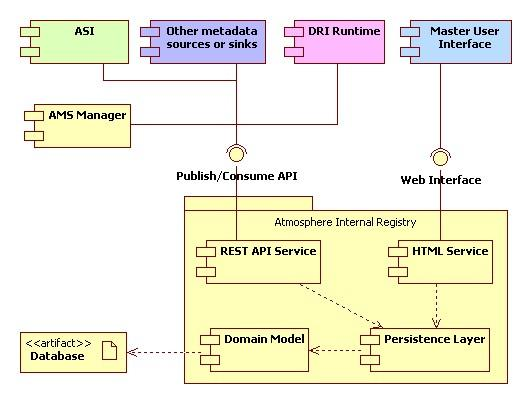
\includegraphics[width=0.7\textwidth]{images/air-architecture.png}
	\caption{The overview of Atmosphere Internal Registry (AIR) component.
	Many VPH-Share core components store and access various metadata in AIR.
	It provides REST API interface for these components, as well as web-based
	html service to enable VPH-Share users to browse the metadata via Master UI
	\cite{vph-deliverable-2-2}.}
	\label{fig:air-architecture}
\end{figure}

From DRI perspective, AIR will store necessary metadata:

\begin{itemize}
	\item \textbf{datasets metadata} and files they contain,
	\item \textbf{integrity checksums} for data validation,
	\item \textbf{service configuration}.
\end{itemize}

Such design enables us to implement DRI as stateless service.

\subsection{Federated cloud storage}
\label{federated-cloud-storage}
Data storage is an essential part of VPH-Share Cloud Platform. The increasing
popularity of cloud storage services due to high quality-cost ratio is leading
more organisations to migrate and/or adapt their IT infrastructure to operate
completely or partially in the cloud. However, as mentioned in section 2.3, 
such a solution has its limitations and implications. To overcome some of 
them one can leverage the benefits of cloud computing by using a combination 
of diverse private and public clouds. This approach is developed in Cloud
Platform as federated cloud storage, where data is stored redundantly on 
various cloud storage services. The benefits are the following:

\begin{itemize}
	\item \textbf{High availability} -- data may be temporarily unavailable 
	and/or corrupted for various reasons when system relies on a single cloud 
	storage provider, as shown in recent cases (see section 2.3). In cloud
	federation we are able to store data redundantly and switch between 
	providers when one becomes unavailable.
	\item \textbf{No vendor lock-in} -- there is currently some concern that 
	a few cloud computing providers become dominant, the so called vendor 
	lock-in issue. Migrating from one provider to another one can also be
	expensive. In cloud federation we are able to easily switch between
	providers considering their charging or policy practices.
\end{itemize}

Federated cloud storage is not sufficient to provide data unavailability 
and corruption tolerance. For this purpose, an additional service
has to be designed to actively monitor data integrity -- DRI.\\

Access to the federated cloud storage is via common access layer -- LOBCDER
service -- served by WebDAV protocol. However, DRI service will access
cloud storage services directly to take advantage of cloud federation and
to omit redundant LOBCDER overhead.

\subsection{Atomic Service}
\label{atomic-service}
In order to ensure smooth deployment for application developers, Cloud Platform
creates a~concept of Atomic Service. It can be simply described as a~VM on which
core components of the VPH-Share-specific application software have been installed,
wrapped as a~virtual system image and registered for usage within the platform. The
process of creating new atomic service is depicted in figure \ref{fig:atomic-service}.
Typical application software installations provided by Atomic Service is federated
storage access, web service command wrapper and web service security agent. Additionally,
Cloud Platform takes care of instantiating various Atomic Services. Atomic Service
Instance is a~specific atomic service deployed on computing resources and providing
VPH-Share application functionality through a~web service (SOAP or REST) interface.\\

Services providing core functionality within VPH-Share will be also deployed as atomic
service instances. 

\begin{figure}[h!]
	\centering
	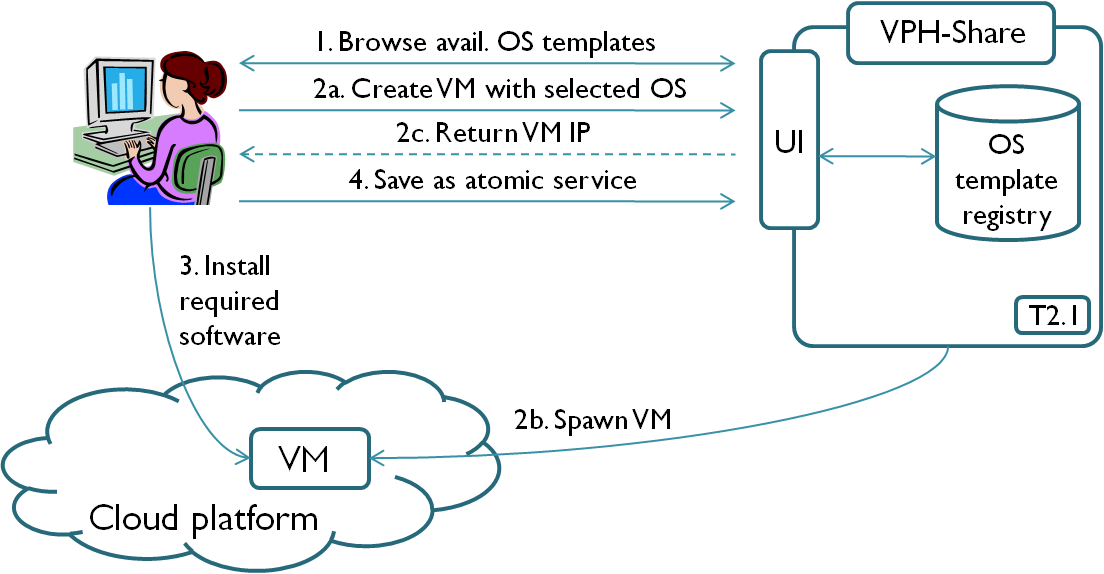
\includegraphics[width=0.8\textwidth]{images/vph-atomic-service.png}
	\caption{The process of creating and instatiating new Atomic Service
	\cite{vph-deliverable-2-2}.}
	\label{fig:atomic-service}
\end{figure}


\section{DRI data model}
The Cloud Platform concerns itself primarily with access to binary data, 
especially via file-based interface. Managed dataset represents a single entity
that can be managed. At its core, it consists of a~selection of
files, to which a portion of metadata is appended and stored in AIR reigstry. 
As data integrity is a crucial requirement of the platform, the datasets can be
tagged for automatic data integrity monitoring (DRI). 

\begin{figure}[h!]
	\centering
	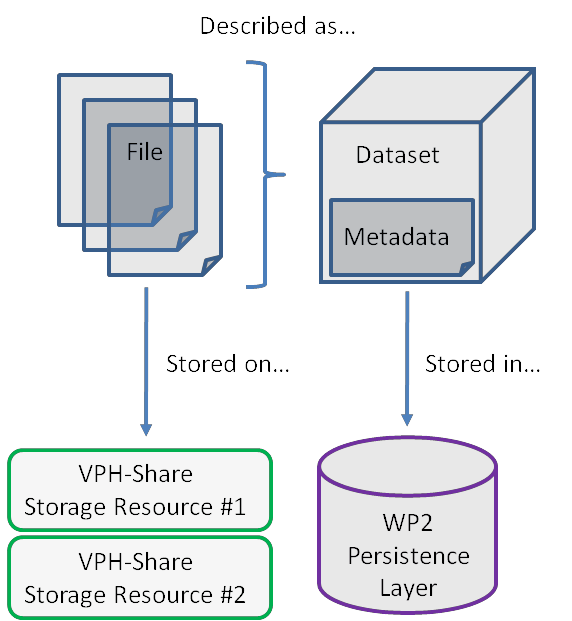
\includegraphics[width=0.5\textwidth]{images/managed-dataset.png}
	\caption{Schematic representation of VPH-Share managed dataset. Managed
	dataset consists of an arbitrary number of files (logical data) that are stored
	on one or more storage resources. The metadata regarding managed dataset is persisted
	in AIR \cite{vph-deliverable-2-2}.}
	\label{fig:managed-dataset}
\end{figure}

\subsection{Metadata schema}
Each managed dataset may consist of an arbitrary number of files (logical 
data) and can be stored on one or more storage resources (data source).
Specific security constraints can be attached to data items, i.e. it cannot be
used in public clouds. In DRI component, validation checks are of configurable
policy (management policy). The schema is depicted in the figure 
\ref{fig:data-model}.\\

\begin{figure}[h!]
	\centering
	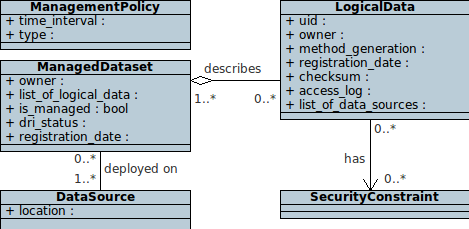
\includegraphics[width=0.8\textwidth]{images/data-model.png}
	\caption{DRI service metadata schema. It generally reflects the concept of
	managed dataset presented in figure \ref{fig:managed-dataset}. Managed dataset
	consists of arbitrary number of logical data and is deployed on one or more
	data sources. Logical data can have security contraints attached to it. Additionally,
	a management policy can be attached to every managed dataset.}
	\label{fig:data-model}
\end{figure}

The managed dataset metadata consists of the following elements:

\begin{itemize}
	\item \textbf{owner} -- reference to user ID of dataset creator,
	\item \textbf{list of logical data} -- list of logical data ids it consists of,
	\item \textbf{is managed} -- marker determining whether dataset's integrity
	is monitored,
	\item \textbf{DRI status} -- dataset's reliability and integrity status,
	\item \textbf{date of registration}.
\end{itemize}

\noindent
Additionally, each logical data will consist of the following attributes:

\begin{itemize}
	\item \textbf{owner} -- reference to user ID,
	\item \textbf{method of generation} -- whether it was uploaded manually, 
	generated by an application or registered externally,
	\item \textbf{date of registration}
	\item \textbf{checksum} -- file's value of a cryptographic hash function
	calculated upon registration and used to validate integrity and 
	availability of file,
	\item \textbf{list of data sources} -- to which the file is currently
	deployed,
	\item \textbf{access log}.
\end{itemize}

While this schema is expected to cover all the requirements addressed in the
DRI service, we foresee that additional metadata can be added later without
affecting already stored.

\subsection{Tagging datasets}
Before automatic verification of managed datasets can take place, it is first
necessary to tag specific data as subject for management. It is foreseen that
the DRI component will involve a user interface extension (portlet-based) to
enable authorised users to tag specific datasets for automatic management. This
interaface will display the existing data storage resources and allow creation
of new managed datasets consisting of selected files.\\

In addition to UI based tagging, the DRI component provides API-level access
for the same purpose, whenever a VPH-Share application (or workflow) needs to
tag specific data as a managed dataset.

\section{Requirements}
\label{requirements}
VPH Cloud Platform puts strong empasis on data storage and availability and
integrity assurance, as it is mostly static medical data of great importance.
To fulfill this goal, it takes advantage of outsourcing data storage. To
achieve high data availability in cases of cloud failure (see section
\ref{cloud-model}) and avoid vendor lock-in issues, it utilizes mixture of
public and private clouds. However, it is still desired to monitor periodically
the availability and integrity of data deployed at cloud storage services. DRI
service was designed under several crucial requirements that dictate its
architecture and potential. This section describes these requirements.\\
	
Cloud Platform requirements can be divided into two groups: functional and
non-functional.

\subsection{Functional}
Functional requirements are related to the core system capabilities that it
is desired to ensure. These are the following:

\begin{itemize}
	\item \textbf{Periodic and on-request validation}: DRI has to periodically
	fetch datasets' metadata from the AIR registry and check the availability
	and integrity of managed datasets. It also has to enable API interface for
	this operation to be invoked by the user on demand.
	\item \textbf{Data replication}: DRI has to enable API interface for data
	replication from one data source to the other. 
	\item \textbf{User notification about integrity errors}: validation and
	replication operations has to be performed asynchronously and the results
	have to presented to the user via suitable notification service.
\end{itemize}

\subsection{Nonfunctional}
Nonfunctional requirements are related to the quality of the core system
capabilities, as it is desired that validation and replication mechanisms are
performed efficiently. These are the following:
\begin{itemize}
	\item \textbf{Bandwidth-efficient validation mechanism}: naive download and
	check technique is infeasible. The main DRI challenge is to design and
	implement efficient data validation protocol without accessing the entire
	file.
	\item \textbf{Scalablility}: as it is foreseen that the amount of data
	stored in Cloud Platform resources will be significant, the DRI has to
	present the ability to scale with the size of data. It is suggested to be
	achieved by deploying many independent DRI replicas. 
	\item \textbf{Configurability}: DRI has to provide API interface or UI
	portlet to configure its most important parameter: validation period. It is
	also desired for the designed validation protocol, to be configurable, to
	be able to adjust error-detection probability.
\end{itemize}

\section{Architecture}
The DRI Runtime is responsible for enforcing data management policies. It keeps
track of managed components and periodically verifies the accessibility and
integrity of the managed data. It operates autonomously as well as on request.
It also interacts and cooperates with the other important Cloud Platform's
components (see section \ref{cloud-platform}) to fulfill its goal. At the core
of the service is an application that periodically polls the AIR registry for
a~list of managed datasets and then proceeds to verify the following:

\begin{itemize}
	\item the availability of each dataset at locations read from the AIR
	registry,
	\item the binary integrity of each dataset (checksum-based validation).
\end{itemize}

The DRI Runtime contacts individual data sources and validates the integrity
and availability of the data stored on these resources. Should errors occur,
the DRI Runtime invokes a notification service to issue a warning message
to subscribed system administrators (typically, the user defined as the 
dataset's owner).\\

\subsection{Overview}
The architecture of the DRI service was mostly influenced by the Cloud Platform
environment (section \ref{cloud-platform}) and the requirements and challenges
it introduces (section \ref{requirements}). Figure \ref{fig:dri-architecture}
presents its overview.\\

\begin{figure}[h!]
	\centering
	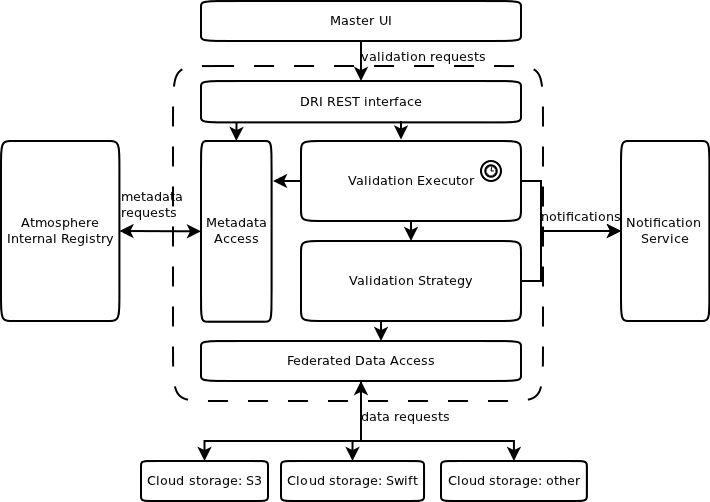
\includegraphics[width=0.8\textwidth]{images/dri-architecture.png}
	\caption{DRI architecture overview. It exposes REST API interface for other
	Cloud Platform components, mostly Master UI. The design is divided into
	modules that are responsible for providing separate functionality.
	ValidationExecution module is responsible for periodical as well as on-request
	based validation of datasets. All of the integrity metadata is provided
	through MetadataAccess module. The complexity of accessing different cloud
	storage providers is abstracted with FederatedDataAccess layer.}
	\label{fig:dri-architecture}
\end{figure}

The DRI Runtime consists of a couple of subcomponents which interact with each
other as well as with other services described. It exposes REST service
interface to be invoked by Master UI or the Atomic Services (see subsection
\ref{dri-interface} for details). MetadataAccess component is responsible for
retrieving necessary metadata from the AIR registry. Access to the federated
cloud storage is performed via FederatedDataAccess layer in order to hide
the underlying complexity and differences between various cloud storage access.
ValidationExecutor represents the core of the DRI. Its objective is to manage
all the validation tasks, both periodical and requested by user. For
each logical data it invokes ValidationStrategy component to perform
its data validation algorithm.

\subsection{Interface and API}
\label{dri-interface}
As hinted upon in the preceding sections, DRI provides end-user interfaces
in the form of a~Master UI portlet, as well as an API implemented by the
Runtime service, where DRI features may be invoked directly by other VPH-Share
intrastructure components.\\

Here we intend to focus on the API, which provides access to the low-level
functionality of DRI and enables it to be configured.\\

As DRI exposes a stateless Web Service, all configuration parameters are stored
in the Atmosphere Internal Registry. Whenever a~configuration change request
is invoked the DRI automatically updates policies stored in AIR. In light
of this, the DRI API supports the following operations:

\begin{itemize}
	\item \textbf{\textit{getDataSources(): DataSourceID[]}} --
	returns a list of currently registered data storage resource identifiers;
	
	\item \textbf{\textit{getDataSource(dataSourceID):
	DataSourceDescription}} -- returns the information on a specific storage
	resource, as stored in the Atmosphere Internal Registry in a form of XML
	document describing the structure of storage resource;
	
	\item \textbf{\textit{registerManagedDataset(DatasetDescription) :
	datasetID}} -- tags a new dataset for management given in
	the form XML document describing the structure of the dataset;
	
	\item \textbf{\textit{alterManagedDataset(DatasetID, DatasetDescription) :
	void}} -- changes the dataset specification stored in the AIR. This action
	should be used to add or remove files from a~managed dataset;
	
	\item \textbf{\textit{removeManagedDataset(DatasetID) : void}} -- excludes
	the specified dataset from automatic management. This does not delete the
	data, it merely stops DRI Runtime from monitoring them;
	
	\item \textbf{\textit{getManagedDataset(DatasetID) :
	ManagedDatasetDescription}} -- requests information on a specific managed
	dataset stored in the AIR, returning XML document specifing the structure
	of the managed dataset;
	
	\item \textbf{\textit{getOwnerManagedDataset(User) : DatasetID[]}} --
	returns a list of user's managed dataset ids;
	
	\item \textbf{\textit{assignDatasetToResource(DatasetID, 
	DataSourceeID) : void}} -- requests DRI to monitor the availability of
	a specific managed dataset in a specific storage resource. If this dataset
	is not yet present on the requested storage resource, it will be
	automatically replicated there;
	
	\item \textbf{\textit{unassignDatasetFromResource(DatasetID, 
	StorageResourceID) : void}} -- requests DRI to stop monitoring the 
	availability of a specific managed dataset on a specific storage resource.
	If the dataset is not present on the selected storage resource, this action
	has no effect;
	
	\item \textbf{\textit{validateManagedDataset(DatasetID) : output}} --
	performs asynchronous validation of the specific dataset and produces a
	document which lists any problems encountered with the dataset's
	availability on the storage resources to which it had been assigned;
	
	\item \textbf{\textit{setManagementPolicy(ManagementPolicy) : void}} --
	changes monitoring parameters. ManagementPolicy is an XML document
	specifying the frequency and type of availability checks performed on
	managed datasets;
	
	\item \textbf{\textit{getManagementPolicy() : ManagementPolicy}} --
	retrieves an XML description of the management policy.
\end{itemize}

\begin{figure}[h!]
	\centering
	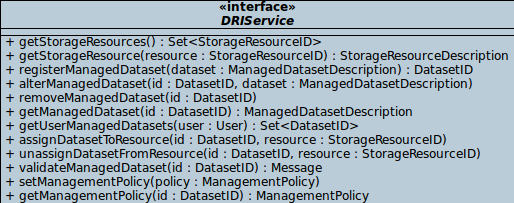
\includegraphics[width=\textwidth]{images/dri-interface.png}
	\caption{DRI Service interface. It provides flexible set of methods to
	manipulate integrity monitoring of datasets.}
	\label{fig:dri-interface}
\end{figure}

Each invocation requires to be augmented by the security token which can be
intercepted and parsed by the security component residing on the virtual
machine on which the DRI Runtime operates.

		\subsection{Typical use cases execution flow}
The two main tasks performed by the DRI is monitoring of data integrity and
replication of managed datasets among various data sources. Now, we will
present a typical execution flow for this tasks through DRI subcomponents
presented in figure \ref{fig:dri-architecture} using sequence diagrams.\\

We start with data validation illustrated in figure
\ref{fig:validation-diagram}. The $validateManagedDataset()$ method is the one
designed to be called by the user, however, the incorporated logic for periodic
integrity checks is the same, as ValidationExecutor fetches all the managed
datasets from AIR and invokes this operation for each of them.\\

\begin{figure}[h!]
	\centering
	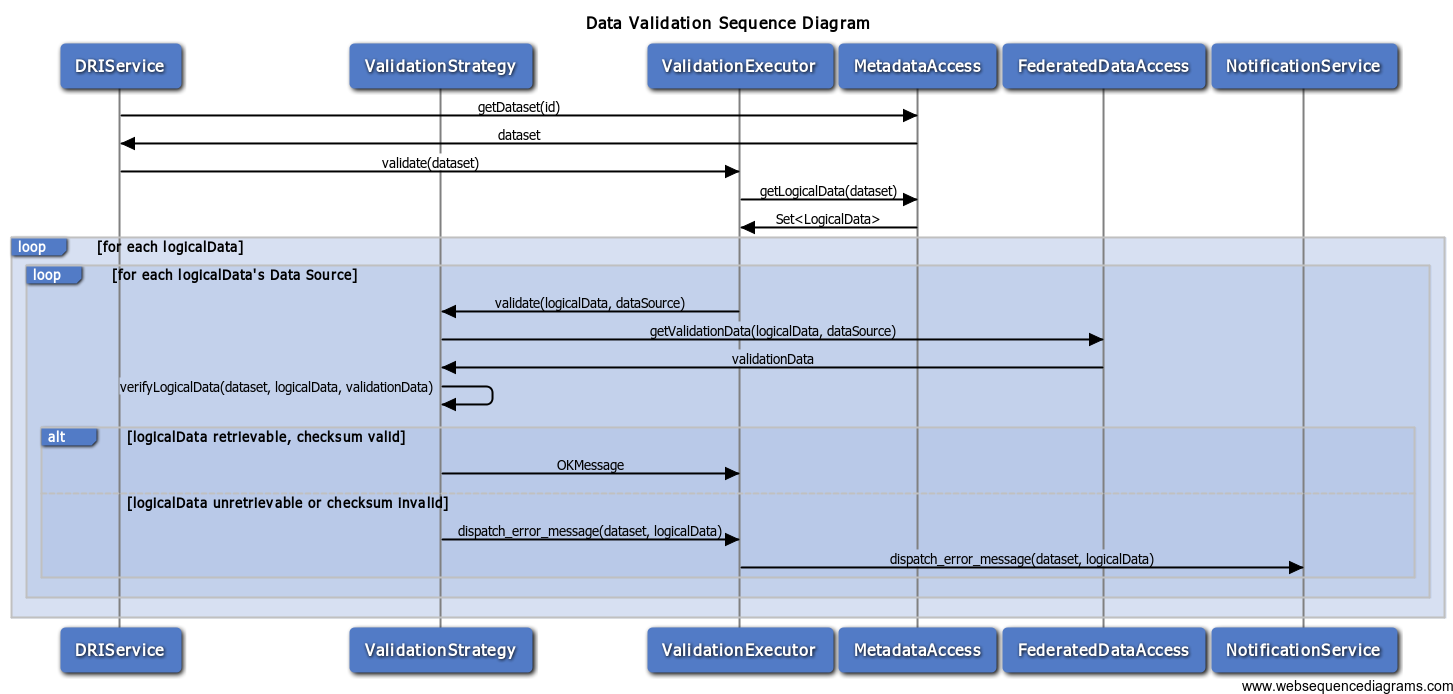
\includegraphics[width=\textwidth]{images/validation-diagram.png}
	\caption{DRI $validateManagedDataset()$ call sequence diagram}
	\label{fig:validation-diagram}
\end{figure}

Upon $validateManagedDataset()$ call, the DRI service retrieves dataset's
metadata from AIR registry invoking $getDataset(id)$ on MetadataAccess object
and passes it to the ValidationExecutor to apply data availability and
integrity check. Subsequently, ValidationExecutor retrieves the metadata of
all the logical data items which are part of the specified dataset invoking
$getLogicalData(dataset)$ on MetadataAccess. Validation occurs separately for
each logical data and against every data source on which it is stored by
ValidationStrategy object which implements efficient validation protocol. To
perform this operation, it has to get some necessary portion of data from data
source by calling $getValidationData(logicalData, dataSource)$ on
FederatedDataAccess object. With this necessary data, ValidationStrategy can
verify whether the specified logical data is available and valid. If not, the
error message is dispatched via NotificationService. It incorporates all or
nothing strategy, which means that the corruption of a single logical data
results in marking whole dataset as invalid. However, detailed error message
informs which items' corruption has been detected on which data sources. The
$validateManagedDataset()$ call performs asynchronously (no return value), but
the result of the operation can be checked via NotificationService.\\

\begin{figure}[h!]
	\centering
	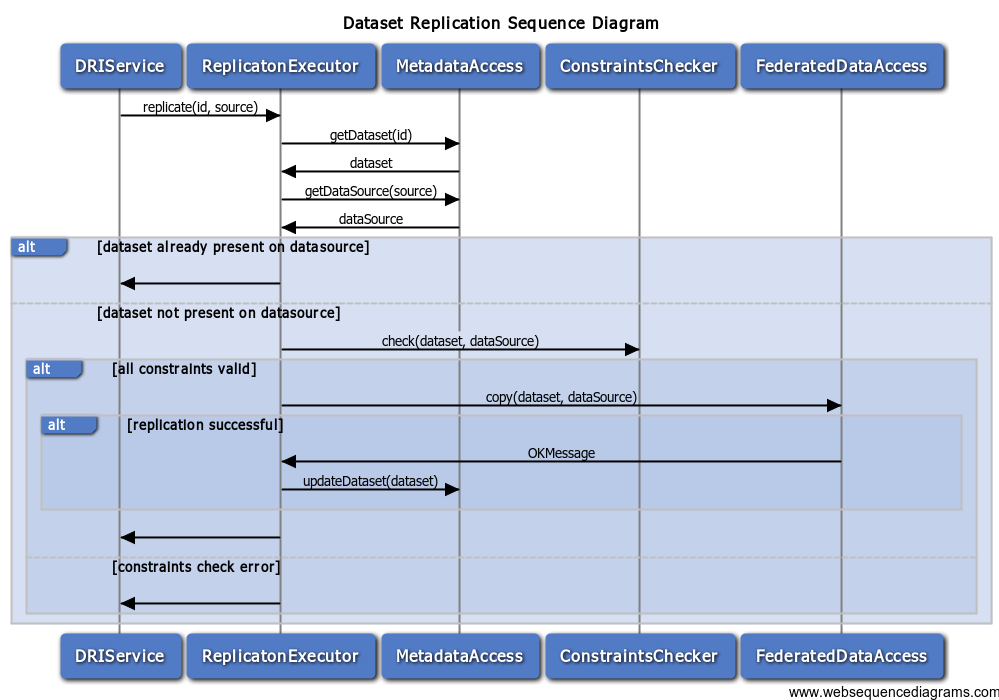
\includegraphics[width=\textwidth]{images/replication-diagram.png}
	\caption{DRI $assignDatasetToResource()$ call sequence diagram}
	\label{fig:replication-diagram}
\end{figure}

Upon \textit{assignDatasetToResource()} 
call (figure \ref{fig:replication-diagram}), the DRIService retrieves
dataset's and data source's metadata from AIR registry invoking
$getDataset(id)$ and $getDataSource(source)$ on MetadataAccess object and
passes it to the ReplicationExecutor. If dataset is already present on the
specified location, this operation has no effect. Subsequently,
ReplicationExecutor checks all the constraints, via 
$check(dataset, dataSource)$ call, that may be associated with the
dataset (such as it cannot be stored in public clouds) and if they are valid,
it performs the replication. This operation simply copies data from one data
source on which the dataset is already present to the specified data source.
In case of any failures, the operation aborts with no side effects. Upon
successful execution, the necessary dataset metadata is updated in AIR registry
($updateDataset(dataset)$ call).\\

	\section{Data validation mechanism}
	\label{section:validation-algorithm}
At the heart of DRI service lies its validation heuristic algorithm which is
going to be described now in detail. As it was discussed in chapter 
\ref{cha:state_of_the_art}, a lot of 
effort was put into ensuring data integrity and availability on storage
resources. However, cloud storage model sets new challenges in this area due to
its constraints and limitations presented in section 2.3. The problem was
addressed in the papers described in section 2.4, one of which - Proofs of
Retrievability - became the basis for many enhancements, modifications and
improvements. Each of the solution approaches difficulties with vast amount of
data stored on cloud storages by creating sophisticated protocols which download
only a fraction of data $(1-10\%)$ and try to guarantee possibly the highest
error-detection rate. Unfortunately, introduced solutions do not address
performance issues of these protocols with regard to typical cloud storage
interfaces and VPH-Share platform requirements:

\begin{itemize}
	\item requesting many small fragments of data greatly affects network
	overhead as each fragment requires separate HTTP request,
	\item cloud storages do not allow executing users' code,
	\item VPH-Share platform requires storing data in unmodified form.
\end{itemize}

These limitations make these solutions impractical. For the needs of DRI
service, a~new approach was designed with practical feasibility and low network
overhead as main objectives in mind. Our heuristic utilizes spot-checking
technique \cite{por, pdp, dip, ric} to verify data integrity with high
probability. Unlike cited mechanisms \cite{dip, por} which generally implement
fine-grained spot-checking, we are aware of cloud storage limitations and
employ coarse-grained spot-checking, realizing that it will result in reduced
error-detection rate.

		\subsection{Algorithm description}
According to the data model described in section 3.1, dataset is a set of files
stored on cloud storage resource. To be able to validate dataset's integrity,
it is firstly necessary to retrieve dataset's data, then compute and store some
checksum metadata for each file. During the validation process, the dataset's
data is retrieved and checksums are computed again to compare them with the
original ones. The following pseudocode illustrates this operation:

\begin{algorithm}[H]
	\SetLine
	\linesnumbered
	\KwData{valid dataset $id$}
	\KwResult{true if dataset valid, error messages otherwise}
	dataset $=$ get$\_$dataset$\_$metadata(id)\;
	files $=$ get$\_$dataset$\_$files(dataset)\;
	\For{file in files}{
		\For{data$\_$source in dataset.get$\_$data$\_$sources()}{
			data $=$ get$\_$validation$\_$data(file, data$\_$source)\;
			\If{data $== null$}{
				dispatch$\_$error$\_$message(file, data$\_$source)\;
			}
			result $=$ validate$\_$data(data, file, dataset)\;
			\If{result is invalid}{
				dispatch$\_$error$\_$message(file, data$\_$source)\;
			}
		}
	}
\caption{Dataset validation algorithm}
\end{algorithm}

To validate a dataset, the metadata of it and all the files it consists of
have to be retrieved (lines 1--2). Then, each file is validated against every
data source it is stored on (lines 3--4). To validate a single file, the
algorithm retrieves its necessary data (line 5). If errors occur, the file's
unavailability message is reported (lines 6--8). Otherwise, integrity checksum
is computed and checked with the original one (line 9). Any resulting integrity
error is reported (lines 10--12).\\

The core part of the validation mechanism is the validation algorithm
(validation protocol) which prepares dataset's metadata and then is able to
validate it. As a typical integrity checking algorithm it comprises of two 
phases: 

\begin{enumerate}
	\item \textbf{setup} -- takes place once (or after each file update) and 
	generates checksum used during every validation phase. During this
	phase the file is divided into $n$ chunks of size $F \over n$ (where $F$
	denotes the size of entire file) and MAC hash is computed for every data
	chunk. Then, a set of $n$ checksums is stored in metadata registry for
	further use.
	\item \textbf{validation} -- takes place on every dataset validation 
	request. During this phase, the file is again divided into $n$ chunks of size $F \over n$ and
	pseudorandom number generator selects $k$ out of $n$ chunk indexes that are
	downloaded and their checksums computed. Then, computed checksums are
	compared with original ones stored in metadata registry.
\end{enumerate}

These phases are graphically presented in figure \ref{fig:algorithm-scheme}.\\

\begin{figure}
	\begin{subfigure}[h!]{0.45\textwidth}
		\centering
		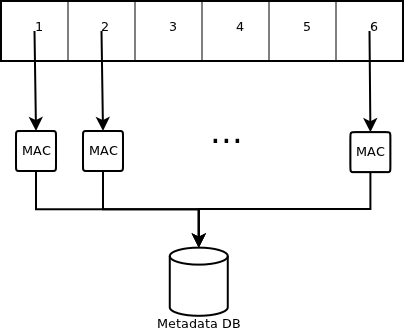
\includegraphics[width=\textwidth]{images/algorithm-setup.png}
		\label{fig:setup}
		\caption{Setup phase}
	\end{subfigure}
	\begin{subfigure}[h!]{0.45\textwidth}
		\centering
		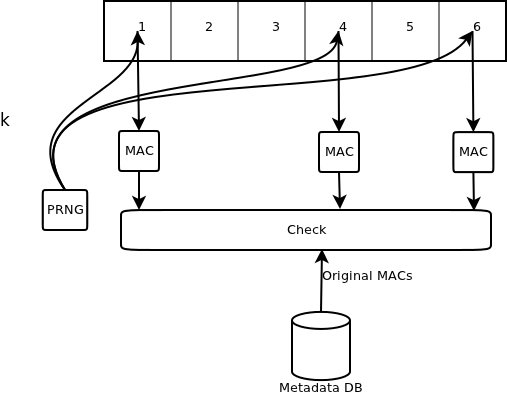
\includegraphics[width=\textwidth]{images/algorithm-validation.png}
		\label{fig:validation}
		\caption{Validation phase}
	\end{subfigure}
	\caption{Single file validation heuristic consists of two phases: setup
	and validation. In setup phase (a), the file is divided into $n$ chunks and
	MAC hash is computed for every data chunk which is then stored in metadata
	registry. In validation phase (b), the file is again divided into $n$
	chunks and pseudorandom number generator selects a set of $k$ out of $n$
	chunk indexes that are downloaded, their checksums computed and compared
	with the original ones stored in metadata registry.}
	\label{fig:algorithm-scheme}
\end{figure}

Values $k$ and $n$ are configurable and can be set to fulfill specified 
requirements. The greater the value of $n$, the smaller the chunks are (see
setup phase description) and more separate $k$ HTTP requests need to be sent to
maintain demanded error-detection rate. With fixed $n$, the greater the value
of $k$, the higher error-detection rate.\\

Datasets consisting of large number of small files can lead to the performance 
bottleneck for two reasons: many separate HTTP requests for each small file and
big storage overhead as chunks are small for small files, but for each a MAC
checksum is stored. For this reason, one additional parameter $threshold$ was 
introduced to improve performance over small files. Data integrity for files
of size smaller than $threshold$ is provided by classic entire-file SHA-256 
checksum. The value of $threshold$ parameter will be established empirically
based on performance test results presented in chapter \ref{cha:testing}.

\subsection{Algorithm analysis}
\label{algorithm-analysis}
Validation algorithm described in the previous subsection is rather simple in 
its design, but poses properties that make it practically feasible:

\begin{itemize}
	\item files are stored in unmodified form,
	\item network overhead and number of HTTP requests can be configured by 
	$n$ and $k$ parameters,
	\item error-detection rate can be configured by $n$ and $k$ parameters.
\end{itemize}

Detailed algorithm description enables theoretical estimation of the most
interesting properties that characterize our solution:

\begin{itemize}

\item \textbf{Error-detection rate} -- expresses the probability to detect data
corruption. For small changes, its value is equal to the probability that the
change took place within the $k$ blocks that are verified:

\begin{equation}
	E_{det} = {k \over n} \hspace{0.6cm} \ for\ small\ changes.
\end{equation}

However, if the prover has modified or deleted substantial $e$-portion of $F$,
then with high probability, it also changed roughly an $e$-fraction of
chunks.

\item \textbf{Network overhead} -- expresses the fraction of data that has to
be retrieved in order to verify the integrity on desired level. As in our
scheme, we download $k$ out of $n$ chunks (each of size $F \over n$), the
network overhead value is proportional to:

\begin{equation}
	N_{over} \sim F \times {k \over n}.
\end{equation}

\item \textbf {Execution time} -- expresses the time needed to validate a file
of size $F$. It depends on average network download speed, as well as on
network latency to the cloud provider. Each HTTP request introduces latency, so
the more requests are sent, the more network efficiency is affected. We
estimate this value in the following way: each chunk
of size $F \over n$ is downloaded in $F \over {n \times speed}$ time (where
$speed$ is download speed in bits/s) plus additional request latency time. As
we validate $k$ chunks per validation phase, we get the execution time: 

\begin{equation}
	T_{exec} \sim k \times ({F \over {n \times speed}} + latency) 
\end{equation}

However, the latency factor can be drastically reduced by performing a set of
HTTP requests concurrently.

\end{itemize}

\begin{table}[h!]
\centering
\begin{tabular}{|l||c|c|}
	\hline
	Metric     & our approach                                           & whole-file approach \\ \hline \hline
	$E_{det}$  & ${k \over n}$                                          & 1 \\ \hline
	$N_{over}$ & $\sim F \times {k \over n}$                            & $\sim F$ \\ \hline
	$T_{exec}$ & $\sim k \times ({F \over {n \times speed}} + latency)$ & $\sim {F \over speed} + latency$ \\ \hline
\end{tabular}
\caption{Performance metrics comparison between our and whole-file approaches}
\label{tab:metrics-comparison}
\end{table}

In table \ref{tab:metrics-comparison} we summarize the three metrics values
for our approach in comparison with whole-file validation approach. Practical
performance evaluation with varying values of the parameters $n$, $k$ and
$threshold$) and in the real cloud storage environment is presented in chapter
\ref{cha:testing}.

\subsection{Summary}
This chapter presented in-depth the design and architecture of data reliability and
integrity (DRI) service. The architecture of the VPH-Share Cloud Platform was introduced
to provide a~context in which DRI is developed and that mostly influenced its requirements.
Given that, we determined the DRI data model and formulated its -- functional and non-functional
-- requirements. The API of the service tries to reflect all of the identified use cases.\\

At the end, we presented the design of the network efficient algorithm that
tries to take cloud storage limitations into account and provide means of network efficient
corruption detection on some level of probability. The concept is based on POR and DIP schemes presented in section
\ref{cloud-integrity-approaches}. Finally, we presented the equations describing the algorithm features.


\chapter{DRI implementation}
\label{cha:implementation}
In the previous chapter, DRI Service architecture was described. In the
following, we present the way how we have implemented it. We also
discuss the technologies that were used for the separate parts of the service.
At the end we briefly descibe how it could be used outside of the VPH-Share
Cloud Platform and integrated in other environment.


\section{Overview}
Implementation of a large software system typically involves some set of
technological or paradigmatic assumptions that have to be taken into
consideration while implementing its components. VPH-Share Cloud Platform takes
advantage of SOA paradigm. All of the components are designed as loosly-coupled web
services that cooperate via REST interfaces. As a~result, each component may
theoretically be implemented using any technology stack. However, to avoid
excessive diversity of software technologies, most of them are implemented in
Java or Ruby programming languages, the practically proven open source
solutions.\\

As it was mentioned in section \ref{cloud-platform}, all of the Cloud
Platform's core services will be deployed within Atomic Service instances,
a VPH-Share application container. Atomic Service can be simply viewed as VM
with add-on software and mechanism installed, such as security or federated
data access layers.\\

DRI Service implementation was conducted according to the architecture
described in chapter \ref{cha:architecture} with the best software development
practices, such as testing and design patterns in mind. The main goal is to
achieve the highest possible data validation efficiency, while providing an
acceptable probability of unavailability or error detection. The design of DRI
Service already solved some performance issues, mostly on the validation
algorithm. However, implementation details have to be taken into account.
	
\section{Challenges and decisions}

It is a recurring engineering truth, that practical implementation to some degree
always affects the design. Ideally, project's implementation should accurately reflect
its design. However, different technology stack choices vary significantly, from
programming language paradigm and available contructs, to best practices and design
patterns, to available libraries and their specifics. Therefore, DRI architecture
presented in chapter \ref{cha:architecture} represents only the the conceptual and
functional view of the service.\\

With DRI Service architecture design we clearly identified the biggest software
engineering challenges that have to be addressed in the implementation. There
are the following:

\begin{itemize}
\item creating REST web service interface (REST producer),
\item REST interoperability with other components (REST consumer),
\item federated cloud access to various cloud storage providers (often non-compatible interfaces),
\item periodic job execution and scheduling,
\item loose coupling between the subcomponents (facilitates configurability and reuse).
\end{itemize}

We have also foreseen, that Cloud Platform components will be changing rapidly
their interfaces and remaining up-to-date will require a lot of integration testing.
It was addressed partially in the DRI architecture, where all of the external service
interactions are wrapped into easily interchangable interfaces (MetadataAccess for example).
Moving with the times, DRI Service implementation was made according to
test driven development (TDD \cite{tdd, tdd-java}) approach to software engineering. 
Broad set of integration sets created this way allowed to spot changes in
other components.

\section{Implementation technologies}
Java programming language \cite{java-language} was chosen as implementation
language and technology stack. Advantages are significant, Java:

\begin{itemize}
\item proved to be high-performance and commercially proven,
\item has a vast number of libraries available,
\item has big and active community,
\item has wealth range of developer tools.
\end{itemize}

At its core, DRI Service is a Java Servlet \cite{java-servlet}
component which accepts REST requests on specified URI paths and performs the
requested task utilizing MetadataAccess, ValidationExecutor, 
ReplicationExecutor, ValidationStrategy and FederatedDataAccess, implemented as
simple Java objects. In Java Servlet model, the programmer is free of the
object's lifecycle management and REST/HTTP communication complexities, which
is provided by the container into which application is deployed.\\

Another important implementation's aspect is dependency injection (DI \cite{di,di-book}). It is
a~software design pattern which releases the programmer from "dependency-hell"
problem. It removes the need to provide dependencies (object instances) when
constructing objects, which is error-prone. Dependencies are provided
dynamically by the DI container at runtime according to the configuration.
In DRI, we use Guice library \cite{guice} for DI capabilities. DI approach
significantly simplifies component's testing in a service-based environment as
dependable service can be simply swapped with a~mock object in the
configuration.\\

DRI Service components implementation technologies are depicted in figure
\ref{fig:dri-impl-technologies}. Further subsections describe them in detail.

\begin{figure}[h!]
	\centering
	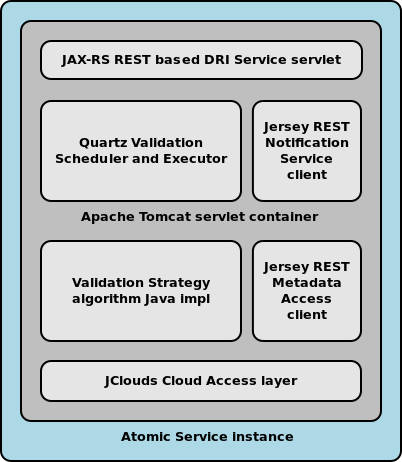
\includegraphics[width=0.5\textwidth]{images/dri-impl-technologies.png}
	\caption{DRI Service implementation technologies of its modules. REST API
	interface is provided using JAX-RS technology. Federated data access is built
	on JClouds library which abstracts the complexity of accessing different cloud
	storage providers. Jersey REST client library eases the integration with REST
	based services on which DRI depends. Finally, in batch execution DRI utilizes
	Quartz library.}
	\label{fig:dri-impl-technologies}
\end{figure}
 
\subsection{REST interfaces}
To provide REST interface and cooperate with other Cloud Platform
components, DRI utilizes Jersey library \cite{jersey} -- a reference
implementation of the JAX-RS specification \cite{jax-rs} and supports seamless
integration with Java Servlet technology. It provides both, server and client
REST interoperability via Java annotations \cite{jls}.\\

\subsubsection{Server side}
In JAX-RS to create a REST interface for DRI it is as simple as the following:
Creating JAX-RS based REST service interfaces is very simple. The following
listing shows a part of the DRIService interface:

\lstinputlisting[language=Java, basicstyle=\footnotesize, frame=single]{src/DRIService.java}

To make your Java method available through REST you simply annotate the class and its methods with
JAX-RS annotations. Let us take \textit{getManagedDataset} method as an example. It will

\begin{enumerate}
\item be available under \textit{/driservice/get\_managed\_dataset/{datasetId}} URL,
where \textit{datasetId} is a string part of the URL specifying dataset id (\textit{Path} annotation),
\item be accessible via HTTP GET method (\textit{GET} annotation),
\item produce HTTP JSON format output (\textit{Produces} annotation).
\end{enumerate}

The format of the \textit{ManagedDataset} JSON method output is mapped into Java object
via \textit{XmlRootElement} and \textit{XmlElement} JAXB annotations \cite{jaxb}.
 
\subsubsection{Client side}
Creating Jersey based client of the REST service is also straight-forward:

\lstinputlisting[language=Java, basicstyle=\footnotesize, frame=single]{src/AIRMetadataRegistry.java}

Here, we use already configured \textit{WebResource} object to build REST query to 
\textit{BASE\_URL/get\_datasets} URL with \textit{only\_managed} query parameter. Jersey
automatically deserialize the returned response into \textit{ManagedDataset} object
we presented in the previous listing.\\

\subsection{Cloud storage access}
Current cloud storage services mostly provide a~standard REST interface.
Despite interface similarities, it appears cumbersome to support the
differences between providers. To get rid of this problem, DRI uses JClouds
\cite{jclouds} library that provides a~common API layer that abstracts cloud
dissimilarities. Thus, access to the cloud storage federation is quite easy
via programmer perspective. At the time of writing this thesis, JClouds
supports up to 30 different cloud providers including Amazon, GoGrid, vCloud,
Openstack, Azure and others. Storage access is provided as Blobstore API, which
incorporates three concepts: service, container and blob. The Blobstore is
a~key-value store such as Amazon S3, where your account exists and where you
can create containers. A container is a namespace for you data and many of them
can exist. Blob is an unstructued data stored in a container referenced by
its name. In all cloud storages, the combination of the account, container and
blob relates directly to the HTTP URL. Access to data can be performed
synchronously or asynchronously, depending on the selected Blobstore type.
While Blobstore API provides cloud storage abstraction it cannot overcome
specific cloud provider's limitations, for example size limits or timeouts
between sensitive operations.\\

JClouds's Blobstore abstraction provides uniform interface to different cloud storage
providers. To use provider \textit{X} one have to create \textit{BlobStoreContext}
for \textit{X}. The following snippet simply shows how to access Amazon S3, create a
container and put a blob into it:

\lstinputlisting[language=Java, basicstyle=\footnotesize, frame=single]{src/jclouds-example.java}

\subsection{Task scheduling}
DRI Service periodically monitors data integrity. Periodic tasks invocation
is a~recurring issue in many IT systems. DRI uses Quartz library \cite{quartz}
for task scheduling and execution. Quartz is a~full-featured open source job scheduling
library that can be integrated with, or used along side virtually any Java
application -- from the smallest to the largest e-commerce system. Its main highlights
are the following:

\begin{itemize}
\item periodic and timer jobs,
\item configurable executors (single thread or pool of threads),
\item templates for creating job task objects,
\item support for job transactions and persistence, 
\item scalable -- from simple to complex schedules for executing tens, hundreds 
or even ten-of-thousands of jobs,
\end{itemize}

DRI Service uses Quartz in the following way: at startup it schedules main (root)
periodic job with specified period, which upon trigger, is responsible for scheduling
one validation job per managed dataset. Apart from periodic validation, the dataset's 
integrity check can be performed on request. In such case, DRI tries to add validation
job for the specified dataset to the schedule. If a~job with the same dataset id
already exists in the queue, nothing happens (double validation is not desired). Otherwise, 
the job with specified dataset id is added to the schedule. Worth mentioning is the fact,
that apart from validation jobs, there are jobs that update dataset checksums whenever its
contents changed and both of them cannot collide with each other. Upon job execution, a
\textit{JobDetail} is returned.

\section{Data validation implementation details}
DRI Service utilizes efficient data validation algorithm to achieve acceptable
performance over large amount of data. However, apart from algorithm
efficiency, its optimized implementation is greatly desirable. Due to the fact
that the validation algorithm is highly oriented on network communication (see
section \ref{section:validation-algorithm}), network bandwidth and latency are
the most significant factors affecting its performance. The point of the
biggest interest is access to large number of the selected chunks of data. As
it was noted in section \ref{cloud-model}, current cloud storage interfaces do
not enable efficient way to perform this operation. However, even though
individual chunks of data have to be requested in separate HTTP calls, they can
be invoked asynchronously in parallel to reduce round-trip time (RTT) latency.
DRI employs this scheme via asynchronous Blobstore API provided by JClouds
library. When DRI validates single logical data within dataset, it invokes
a~configurable number of asychronous data chunks requests and then waits for
their completion. The scheme repeats until all the needed chunks for logical
data are collected.\\

\section{Deployment environment}
Currently, at proof of concept stage, the DRI is deployed on Apache Tomcat
\cite{apache-tomcat} instance which runs on virtual machine (VM). However, in
full-operational Cloud Platform it will be deployed within Atomic Service
instance (simply a VM with some add-ons) as one of its core services. Apache
Tomcat is a web application container which implements Java Servlet
specification and provides its application environment. Nevertheless, any other
application server compliant with Java Servlet specification can be used.

\section{The use outside of Cloud Platform}
DRI Service component could be successfully used outside of the VPH-Share Cloud Platform
frame. By design, its dependent components are used through abstraction layers and could
be easily swapped to accomodate to other environment. Metadata could be stored on
cloud storage or local disk file; Notification Service could be implemented as a mail sender
or chat client -- every such change requires only to modify one package (see figure 
\ref{fig:dri-ability-to-change}. Moreover, many of the configuration parameters such as:
REST urls, credentials, federated cloud metadata etc, are kept in configuration file and
can be easily changed.

\begin{figure}[h!]
	\centering
	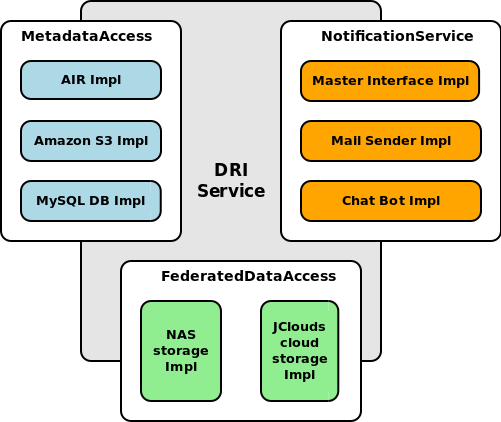
\includegraphics[width=0.6\textwidth]{images/DRI-ability-to-change.png}
	\caption{Possibility to switch DRI service providers by reimplementing abstraction
	layer and accomodate to new environment, other than VPH-Share Cloud Platform}
	\label{fig:dri-ability-to-change}
\end{figure}

\section{Scalability} 
It is foreseen, that with the growth of the platform it could be necesarry for DRI to
provide scalable solution. Hopefully, by design, DRI is a stateless web service so the
simplest solution would be to run a couple of its instances and provide requests load
balancing between them. Another possibility, as DRI uses Quartz for job scheduling and
execution, would be to build Quartz cluster and make DRI submit its validation jobs
to it. Lastly, single dataset (or even single file) validation is completely independent
from one another, meaning that scalability issues can be easily addressed.

\section{Summary}
This chapter presented the way DRI service was implemented based on its design and
requirements described in the previous chapter. It outlines the choice of Java technology stack
and additional libraries and justifies it. JClouds library helped us to address one of the
main implementation challenges to abstract cloud storage access and get rid of cloud provider
interface differences. Additionally, JAX-RS, Guice and Quartz enabled us to create the skeleton
of DRI implementation relatively fast and without complications. At the end we also discuss
the possiblitity to use DRI outside of VPH-Share platform. To achieve this, one has to reimplement
the abstract layer through which DRI accesses external services. On the other hand, scalability can
be easily achieved by small modifications through running multiple instances of DRI service and
pinning datasets periodical validations to concrete instances.

\chapter{Verification and testing}
\label{cha:testing}

	\section{Functional requirements verification}
A key aspect of the DRI service is to meet its requirements within Cloud
Platform, which were listed in section \ref{requirements}. In the prototype
phase, we are focusing mostly on data validation. As project continues, data
replication mechanisms will be developed within DRI service. As previous
chapters shown, we designed and implemented a service which enables periodic
and on-request data validation and notifies about any integrity or availability
errors. It can be used according to the REST interface described in chapter
\ref{cha:architecture}.\\

In future Cloud Platform releases Notification Service depicted in figure
\ref{fig:dri-architecture} will provide notification functionalities for the
platform. In our prototype, we developed simple mock for this important
component in the form of a webpage. Its sample view during normal operation is
presented in figure \ref{fig:notification-service}.

\begin{figure}[h!]
	\centering
	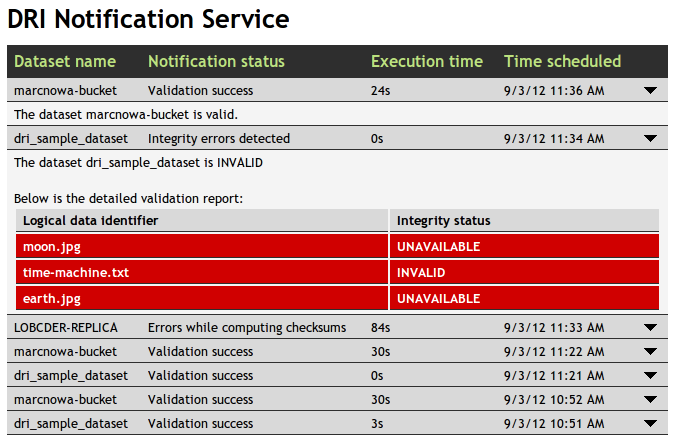
\includegraphics[width=0.8\textwidth]{images/notification-service.png}
	\caption{Notification service mock -- sample view}
	\label{fig:notification-service}
\end{figure}

Here we can see a tabular view of the notifications. A notification
is represented by one row and is always associated with single dataset.
Each row presents basic information: 

\begin{itemize}
\item dataset name,
\item notification status -- short message informing whether operation
(compute/validate) succeded or there were some errors,
\item execution time -- the time it took to perform the operation,
\item time scheduled -- the time when the operation started.
\end{itemize}

Additionally, when the user is interested to see more details about the operation,
he can just expand the row with a click. In figure \ref{fig:notification-service}
we can see \textit{dri\_sample\_dataset} expanded and detailed information about the
integrity errors that occured.

	\section{Efficiency metrics}
		\subsection{Network bandwidth}
		\subsection{Error detection rate}
		\subsection{Scalability}
	\section{Efficiency tests}
		\subsection{Environment description}
		\subsection{Experiments}
		\subsection{Results}
	\section{Other nonfunctional requirements verification}
	\section{Conclusions and results}

\chapter{Summary and future work}
\label{cha:conclusions}

The main objective of this thesis was creation of a~data reliability
and integrity (DRI) service that monitors the availability and integrity
of data stored on heterogeneous cloud storage resources. As it was shown,
the resulting advantages of moving the data to the cloud suggest that widespread
use of cloud storage seems inevitable. However, this new approach is not free
from dangers. Recent cloud provider failure and malicious corruption reports
\cite{amazon-downtime1, amazon-downtime2, gmail-downtime, docs-downtime} 
show that
one cannot fully entrust the data to the cloud provider. But cloud storage brings
new challenges for ensuring data security. Therefore, computer industry seeks for
innovative tools and methods that could lower the risk associated with the current
trend. The idea oscillates around harnessing multiple cloud storage providers
and replicate the data among them. This approach creates a~new layer of abstraction
in accessing the data -- cloud storage federation. While storing many copies of 
data on different cloud providers significantly reduces the risk of data loss, it
is still needed to detect data problem. Hash-based checksums and error correcting codes
are the industry standard methods of ensuring data integrity. However, cloud storage
introduces obstacles against applying them, because data is stored remotely and cloud
providers charge fees for outbound network transfer. As a~result, for instance, 
validating a~file by computing its SHA-512 hash based on the full content of it can
significantly raise operational costs. Additionally, network latency and throughput
affect the data access.\\

In this work different approaches for ensuring data integrity in cloud storage were
presented. On-going research effort focuses on selectively validating the content of
data and detecting corruption only on some level of probability. Discussed validation
schemes propose different improvements of the outlined approach such as encrypting
the content of data or they assume the existence of the element that performs computation
on data without transfering it to the verifying peer. However, in the scope of VPH-Share
project, the data stored on remote cloud resources cannot be altered, as well as no
computing element exist on cloud provider site.\\

As a~result, in this thesis we aim to address the above mentioned issues with
creation of a~service that is periodically monitoring the availability and integrity
of data and notifies the owner in case of errors. It was successfully designed,
implemented and deployed in production environment of VPH-Share project. However,
at this stage of project, DRI is a~work in progress and not all of its requirements
outlined in VPH-Share deliverable are already met. The core functionality is up and
running, but data replication mechanisms are scheduled for the second phase of the
project. Nevertheless, this thesis objectives have been evaluated and the results
of executing a~test scenario were outlined in the chapter devoted to verification
and testing.

\section{Future work}
While working on this thesis, we identified some ideas and tasks that are connected
to this work, but were not taken into consideration. However, they could be worth
continuation, so we outline them here. We divided them in two groups. The first presents
possibilities of enhancements and improvements to this work:

\begin{enumerate}
\item Design and implementation of automatic data replication module. The idea
is to take advantage of and combine both data replication and validation. As soon as
DRI discovers integrity errors, it will recover from them automatically by restoring
the data from other, non-affected replicas. During data recovery, corrupted replica
should be excluded from set of replicas available to VPH users.

\item Investigation and implementation of possible improvements to the validation
algorithm. At the time of writing this thesis, cloud storage interfaces are of
limited flexibility. Every noncontiguous block of data has to be requested with 
separate HTTP request. It can significantly affect the efficiency and throughput
of validation algorithm. In the current implementation, DRI asynchronously sends
a~set of HTTP requests to reduce network latency. If cloud providers introduced
support for requesting multiple noncontiguous blocks of data in single HTTP call
or for emerging SPDY web protocol, it would be beneficial to add support for it
in DRI. Another idea it to perform data validation against multiple cloud providers
simultaneously. Separate blocks of data should be reqested from different replicas.
Other implementation improvements could also be investigated.

\item Design and investigation how to combine DRI with LOB federated data access
(LOBCDER) into one component. LOBCDER provides federated data access for the VPH-Share
Cloud Platform -- all the requested data flows through this component. Many limitations
to DRI design came out from separating these two components by design. In case of
ensuring data integrity the combined component could perform data validation
on the fly as the data is requested and retrieved from cloud storage. When data corruption
occur, it could automatically recover by restoring the data from the remaining replicas.
Moreover, it could perform data encryption while storing in the cloud. As a~result,
validation algorithm would not be constrained with the requirement to store the data
in original form, as well as it could be substituted with proofs or retrievability
scheme.
\end{enumerate}
 
The other group addresses the problem of ensuring data integrity in cloud storage
in general and abstracts away from VPH-Share project context. The concept monitoring
data integrity in DRI service has a~potential for being applied as a~part of many
software solutions. The ideas in this group are the following:

\begin{enumerate}
\item Extract the implementation of data validation mechanism and abstract it away
from the context of VPH-Share project. It would be beneficial to take out DRI
functionality and share it as open source solution. Needless to say that its architecture
should be redesigned and implementation refactored. The design should clearly specify
its dependencies and provide a~couple of implementations out of the box. Currently,
DRI has two core dependencies -- metadata registry and notification service. Metadata
registry stores all the metadata related to data validation and as such could be
implemented as file, database (relational or no-sql) or stored itself on cloud storage
in encrypted form. Notification service informs the user about discovered data integrity
problems and could be implemented in form of email sender, XMPP protocol bot or sms
gateway. Validation algorithm should also be pluggable as different use cases have 
different requirements and limitations.

\item Explore new ways of ensuring data integrity in cloud storage or design a~new
validation algorithm that would satisfy the requirements outlined in this thesis. It is
an on-going research in this field as no standards ways of monitoring data integrity in
the cloud emerged.
\end{enumerate}

The above future work suggestions provide only a~brief description and probably does
not exhaust the subject. However, they are provided as an~inspiration for the broad
spectrum of improvement possibilities.


% itd.
% \appendix
% \include{dodatekA}
% \include{dodatekB}
% itd.

\bibliographystyle{plainurl}
\bibliography{biblio}
%\begin{thebibliography}{1}
%
%\bibitem{Dil00}
%A.~Diller.
%\newblock {\em LaTeX wiersz po wierszu}.
%\newblock Wydawnictwo Helion, Gliwice, 2000.
%
%\bibitem{Lam92}
%L.~Lamport.
%\newblock {\em LaTeX system przygotowywania dokumentów}.
%\newblock Wydawnictwo Ariel, Krakow, 1992.
%
%\bibitem{Alvis2011}
%M.~Szpyrka.
%\newblock {\em {On Line Alvis Manual}}.
%\newblock AGH University of Science and Technology, 2011.cccccc
%\newblock \\\texttt{http://fm.ia.agh.edu.pl/alvis:manual}.
%
%\end{thebibliography}

\end{document}
